\chapter{TileLink: A Protocol Substrate for Coherence Policy Transactions }
\label{c.tilelink}

TileLink is a protocol framework designed to be a substrate for a set of cache coherence transactions
that implement a particular cache coherence policy within an on-chip memory hierarchy.
Its purpose is to orthogonalize the design of the on-chip network and the implementation of the cache controllers from the design of the coherence protocol itself.
This separation of concerns improves the modularity of the HDL description of the memory hierarchy,
while also making validation and verification of individual memory system components more tractable.

Any cache coherence protocol that conforms to TileLink's transaction structure can be used interchangeably alongside the physical networks and cache controllers we provide.
By supplying a framework to apply transactional coherence metadata updates throughout the memory hierarchy, TileLink enables simplified expressions of the coherence policies themselves.
Conversely, as long as newly designed controllers and networks make certain guarantees about their behavior,
system-on-chip designers can be confident that incorporating them into their TileLink-based memory hierarchy will not introduce coherence-protocol-related deadlocks.
As part of the Rocket Chip Generator project, I have supplied an initial library of cache controllers and physical networks that conform to this TileLink specification.

TileLink is roughly analogous to the data link layer in the IP network protocol stack, but exposes some details of the physical link necessary for efficient cache controller implementation.
This tradeoff avoids imposing any deserialization overhead on data being refilled between levels of an on-chip cache hierarchy, while also allowing for data bus widths
that are tractable to place-and-route between the different caches in the hierarchy.
Despite the emphasis on on-chip deployment, TileLink is suitable for implementing a coherence protocol in a multi-chip system as well.

TileLink is designed to be extensible and supports a growing family of custom cache coherence policies implemented on top of it.
TileLink also codifies a set of transaction types that are common to all protocols.
In particular, it provides a set of transactions to service memory accesses made by agents that do not themselves have caches containing coherence policy metadata.
These built-in transactions make TileLink a suitable target for the memory interfaces of accelerators, co-processors and DMA engines,
and allow such agents to automatically participate in a global shared memory space.

TileLink is hierarchical, in that protocols based on it can be nested inside one another.
This structure comports well with the tree-based structure of on-chip cache hierarchies.
Memory requests that cannot be satisfied within a particular hierarchy level are translated into the protocol assigned to the next-outermost level. 
TileLink uses a variation on the Manager-Client Pairing framework to provide encapsulation and translation between levels.

The rest of this chapter lays out the case for TileLink and provides a detailed specification of its architecture.
I discuss the assumptions and guarantees made by the various components of a TileLink system and explain how components implementing them interact
to supply deadlock and starvation-free, coherent, global shared memory implementations.
Details of how specific coherence policies extend TileLink are discussed in Chapter~\ref{c.coherence}.

\section{Background}

In a system with hardware-managed cache coherence, the cache controllers and memory controllers
communicate among themselves according to some protocol to maintain coherence.
While they might have vastly different implementations, 
all such protocols maintain coherence by ensuring the same {\em single-writer, multiple-reader} (SWMR) invariant \cite{sorin2011primer}. 
For a given block of cached memory, at any given moment in logical time, there is either: 
(1) a single core that may write and read the block, or 
(2) there are zero or more cores that may only read the block.
However, because this definition is based on a notion of logical time rather than physical time,
it does not preclude a variety of important optimizations that would otherwise appear to violate this constraint.
Our definition of coherence must also augment the SWMR invariant with a data value invariant
that pertains to how values are propagated from one logical epoch to the next.
This invariant states that the value of a memory location at the start of an epoch
is the same as the value of the memory location at the end of its last read-write epoch \cite{sorin2011primer}.
Violating either of these invariants could lead to values stored out by one core never becoming visible to other cores.

For the rest of this chapter, I distinguish coherence policies from coherence protocols.
A coherence {\em policy} governs how the SWMR invariant is represented as metadata identifying available permissions on data blocks.
A coherence {\em protocol} specifies the exact flows of messages and state updates that must be propagated through the memory hierarchy in order to effect a policy.
In other words, a policy specifies what access permissions are possible and when those permissions should be changed,
whereas a protocol specifies how any changes are communicated to the rest of the hierarchy.
TileLink provides a single coherence protocol {\em template} on top of which many policies can be implemented.
A particular cache coherence policy will specify permissions changes that must occur as a result of a serialization of memory operations.
Using these policy-based decisions to fill in the TileLink template results in a complete coherence protocol.

A protocol is made up of a specified set of allowable interactions between any agents that store and request copies of blocks of shared memory.
We term legal sets of interactions between agents ``transactions'' because the SWMR invariant must be preserved,
even though the permissions metadata is distributed throughout the hierarchy.
Futhermore, all clients must agree on the serialization of permissions changes to a particular block.
The distributed agents must achieve consensus about permissions and data despite the fact that there may be no ordering guarantees
provided by the underlying communication network, and so no trivial notion of global serialization of the transactions.

The transactions that make up a coherence protocol tend to assume a particular shape depending on what
assumptions are built into the underlying message transport network they rely upon.
Figure~\ref{fig:hops} shows how certain transport assumptions result in different numbers of messages sent per transaction and different points of serialization.
In Figure~\ref{fig:hops}.A, by exploiting a globally synchronous broadcast medium (such as a bus), client agents can directly reply to one another in only two hops.
When only point-to-point communication is available (Figure~\ref{fig:hops}.B), a manager agent provides a possible point of synchronization, as well as forwarding certain filtered messages to other clients.
However, those clients then respond to the transaction originator directly.
If the point-to-point network cannot guarantee ordered message delivery, transactions can include a fourth hop (Figure~\ref{fig:hops}.C)
that will add latency, but which provides opportunities for more fine-grained concurrency control to maintain a global serialization.
The symmetry of a four-hop transaction style also enables hierarchical composability in multi-level memory systems.
TileLink is based around a four-hop structure.

\begin{figure}[t!]
\centering
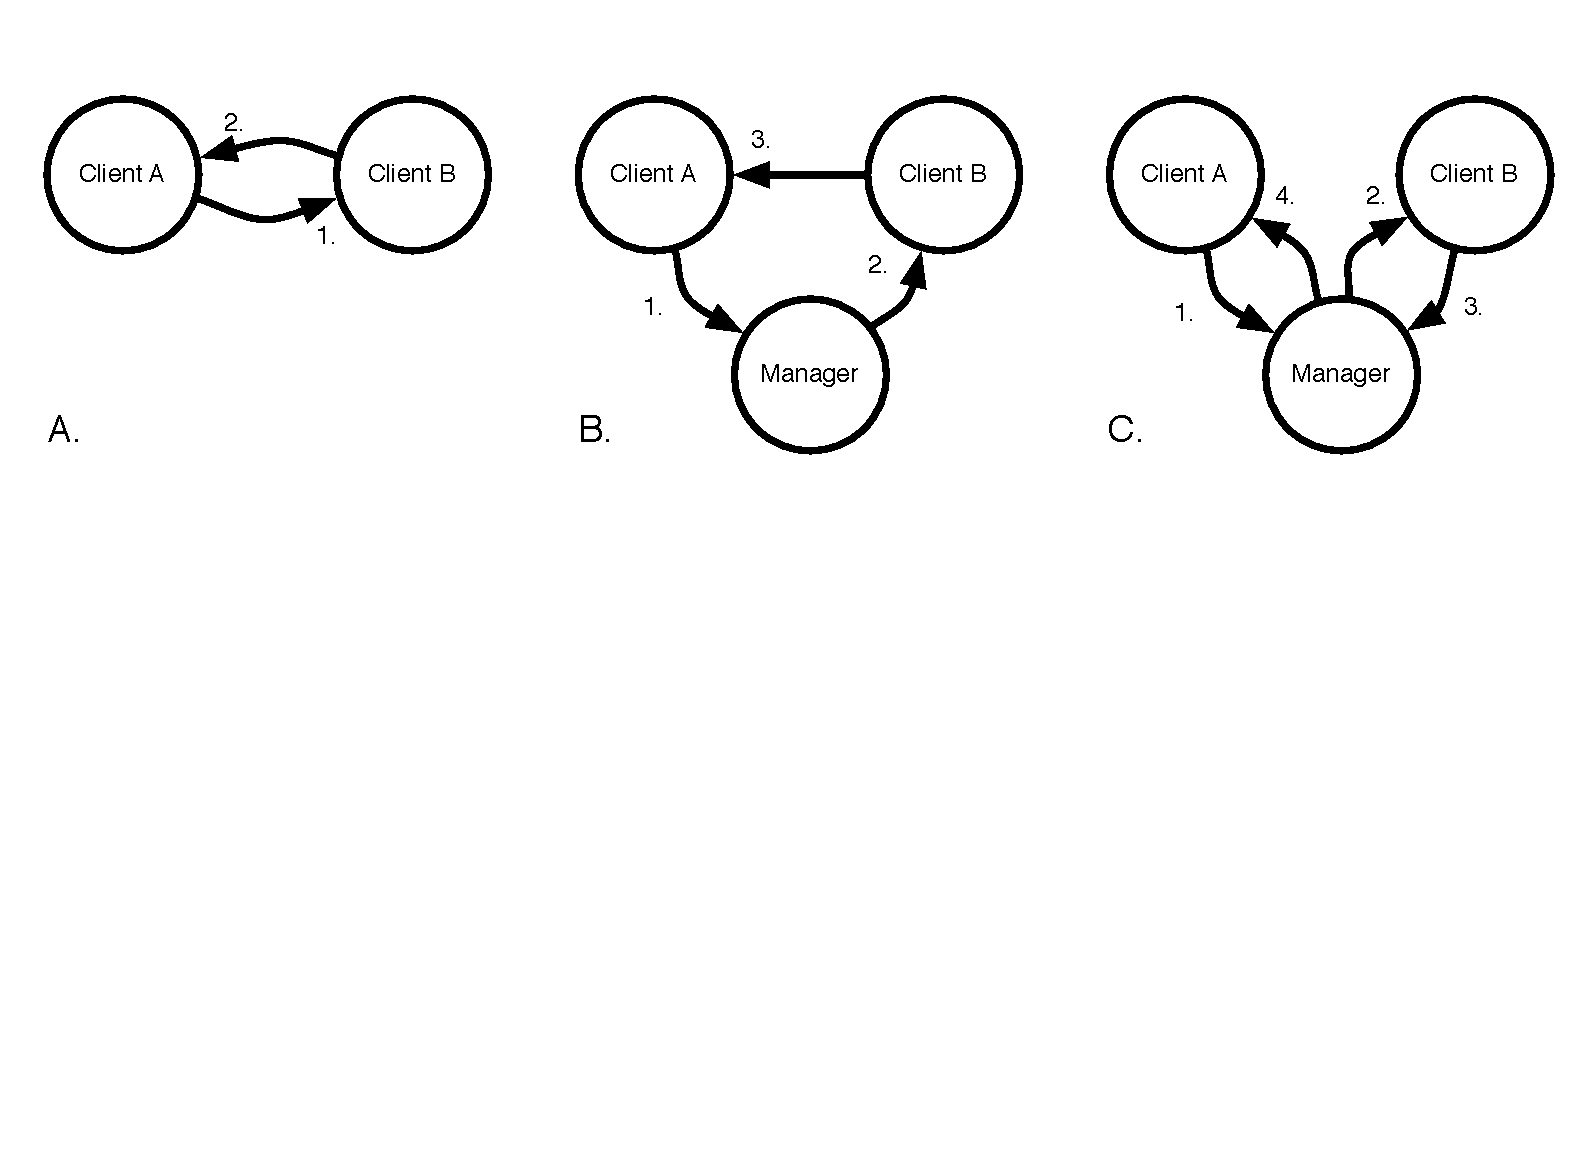
\includegraphics[width=1\columnwidth]{tilelink/figures/hops.pdf}
\caption[Sketches of various coherence transaction shapes.]{
Sketches of various coherence transaction shapes.
A. Exploiting a globally synchronous broadcast medium, client agents can directly reply to one another in two hops.
B. With point-to-point communication, a manager agent provides a possible point of serialization.
C. With unordered message delivery, a fourth hop can symplify the complexity of maintining a global serialization.
}
\label{fig:hops}
\end{figure}

Thus far we have discussed the concepts that inform the behavior of TileLink within a single level of the memory hierarchy.
In order to extend TileLink to support protocols that span multiple levels of the hierarchy, we apply a variation of the Manager-Client Pairing (MCP) framework \cite{beu2011manager}.
MCP defines an interface between users of data (client agents) and the mechanisms that monitor coherence of these users (manager agents) on the two sides of a coherence protocol interface.
A given agent can act also as both a client and a manager, and serve as the bridge between two nested realms of the multi-level coherence protocol.
Figure~\ref{fig:mcp} shows how this strategy can be applied in a divide-and-conquer manner to arbitrarily deep hierarchies
by carving them up into nested coherence realms.
Applying the MCP framework to a memory sytem is advantageous because it provides
encapsulation within each tier of the hierarchical protocol,
which in turn mitigates the state space explosion
that makes multi-level protocol designs prohibitively expensive to verify.
Standardization and encapsulation enable more rapid
design of hierarchical coherence protocols via community-validated
building blocks that can be readily compared, tested and evaluated \cite{beu2011manager}.

\begin{figure}[t!]
\centering
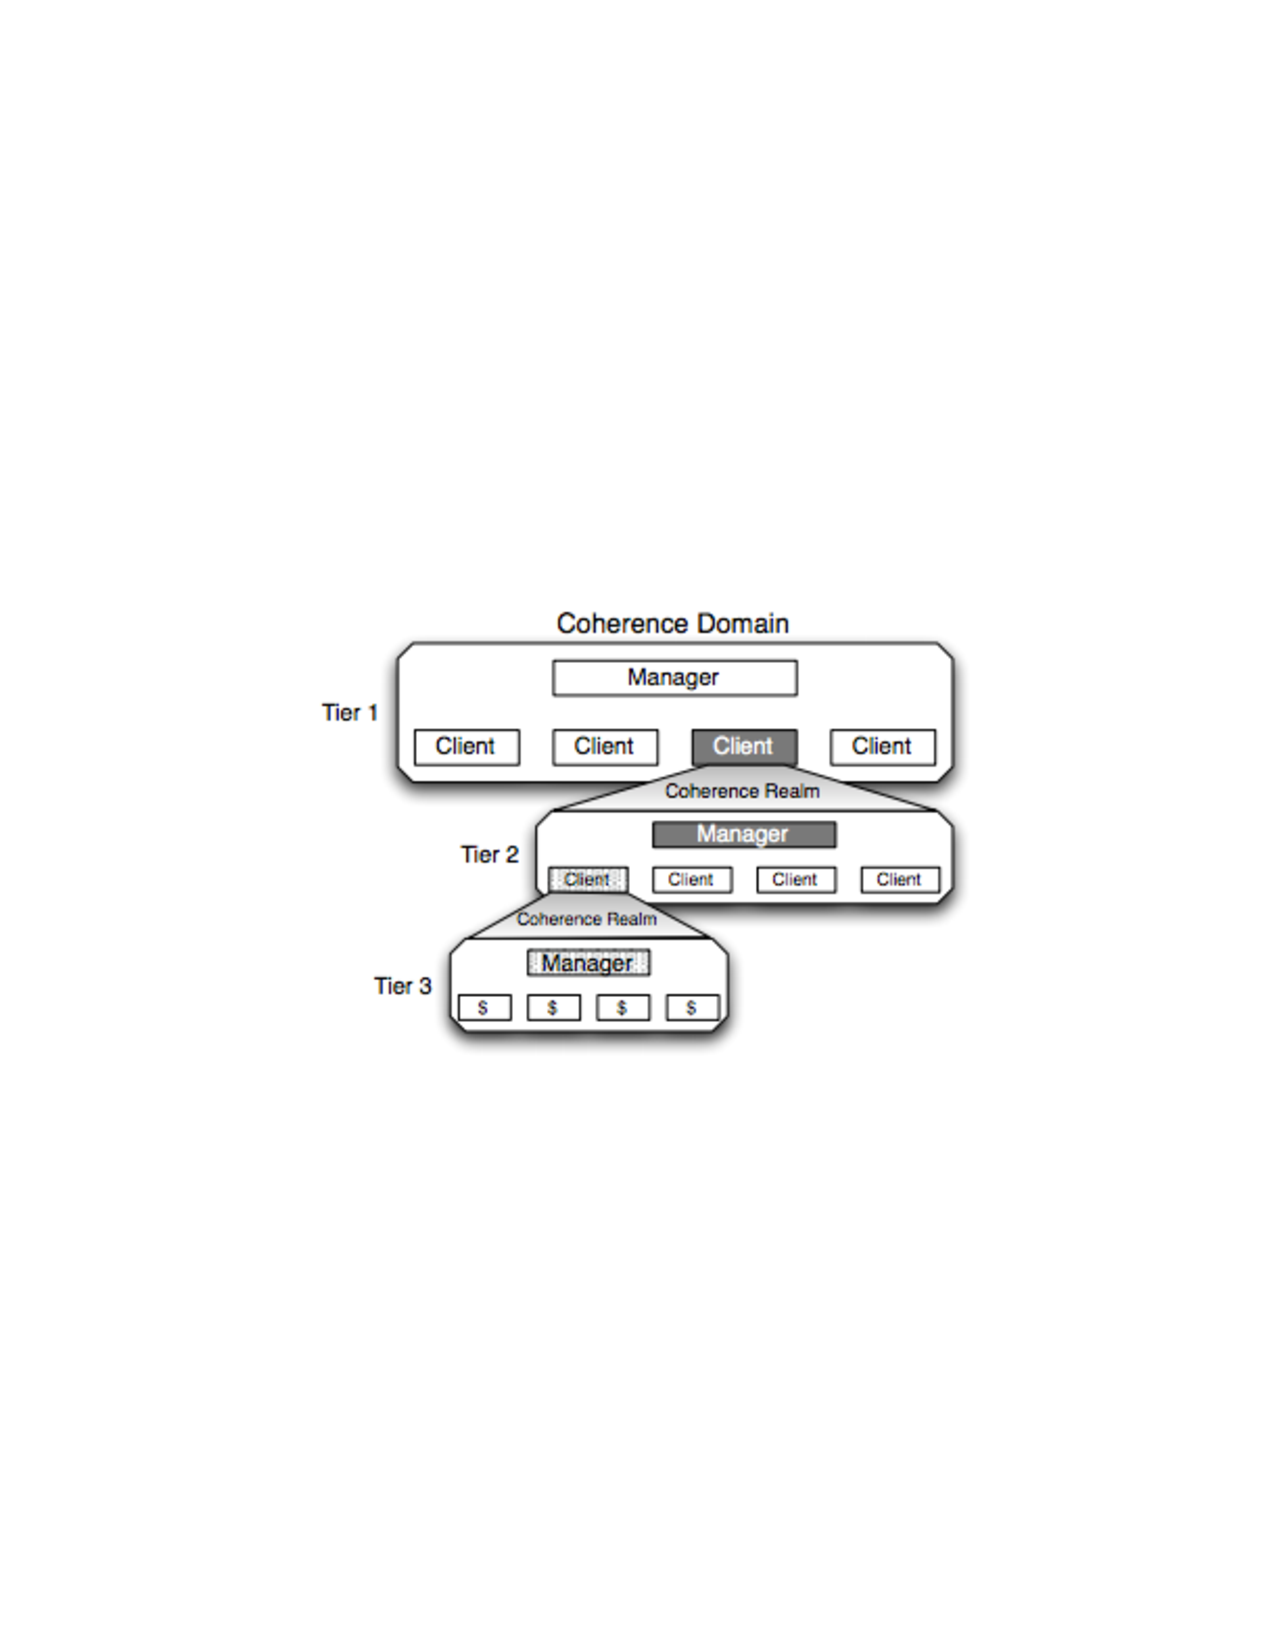
\includegraphics[width=0.8\columnwidth]{tilelink/figures/mcp-realm.pdf}
\caption{Nested coherence realms in the MCP paradigm. TODO }
\label{fig:mcp}
\end{figure}

\section{Architecture}
\label{s.arch}

The fundamental components of the Tilelink specification are agents, channels, and transactions.
{\em Agents} are the active participants in the protocol that send and receive messages in order to transfer copies of data through the memory hierarchy.
Five independent {\em channels} transfer messages containing metadata and data between agents.
A {\em transaction} is a specific sequence of messages sent between agents via these channels
that cause certain agents to gain or lose permissions to access copies of cached data blocks.

TileLink is a hierarchical protocol, wherein a Manager-Client Pairing (MCP) methodology encapsulates the complexity of supporting
multiple levels of protocol within a single memory hierarchy~\cite{beu2011manager}.
Within any one level of the memory hierarchy, TileLink is based off of a symmetric, four-hop transaction structure (Figure~\ref{fig:hops}.A).
Manager agents serve as a point of serialization for coherence transactions on a block occuring within their coherence realm.
All messages sent to clients are eventually acknowledged, which allows the manager to ensure that all clients have
individually serialized transactions on a particular cache block in the same order.

TileLink tries to impose as few constraints as possible on the implementation of both the agents' controllers and the underlying physical network.
This design emphasis somewhat increases protocol complexity, but it makes TileLink applicable to a wide variety of physical design constraints and application domains.
With regards to agents, TileLink does not make assumptions about what state the agents are capable of storing about each cache block,
though it does require agents without state to operate in particular, conservative ways.
TileLink does not assume that messages are delivered in order between two particular endpoints by the underlying physical network,
though it does require an extra transaction message absent point-to-point ordering.
The ramifications of these design decisions are discussed in more detail in the following sections.

\subsection{Agents}

Agents are the active participants in the protocol that send and receive messages in order to transfer copies of data through the memory hierarchy.
Agents participating in the TileLink protocol are either:
\begin{description}
\item[Clients] that request permissions to read or write data within cache blocks, or
\item[Managers] that oversee the propagation of cache block permissions and data.
\end{description}

A client may be a cache, a DMA engine, an accelerator, or any other component that would like to participate in performing memory operations that target the coherent abstraction of global shared memory.
Even clients that do not actually cache a copy of the data within themselves may use TileLink in order to see a coherent view of memory with respect to other clients that do have caches
(i.e., to see dirtied data currently stored in those clients, see Section~\ref{s.uncached}).
Clients are responsible for initiating transactions to gain or cede permissions on copies of cache blocks, and also for reporting on whether they possess certain permissions on those blocks
at the behest of their manager.

A manager may be an outer-level cache controller, a directory, or a broadcast medium such as a bus controller.
Managers may or may not posses a local copy of a data block themselves, but they must know how to source and supply data in response to their clients' requests.
In addition to supplying data, managers are responsible for tracking which clients have been granted which permissions on a data block,
and for probing those clients in order to ensure that the 
single-writer, multiple-reader (SWMR) invariant \cite{sorin2011primer} is upheld.
If a manager does not track the propagation status of individual blocks in precise detail it must be pessimistic
in terms of the quantity and type of probe messages that it sends.
A manager also provides a point of serialization for coherence transactions
initiated by any of the clients within its domain.

In a multi-level memory hierarchy with multiple nested realms of TileLink protocols, a particular agent can function as both
a client (with respect to caches further out in the hierarchy)
and a manager (with respect to caches closer in to the processors).
We term such an agent {\em hierarchical}.
These hierarchical agents must perform a translation of the various message types between the inner and outer protocol.
This translation process is described in more detail in Chapter~\ref{c.coherence}.
Hierarchical agents may or may not store a copy of the data locally, but they must at least track a set of ongoing transactions and serve as a serialization point for the inner protocol.

\subsection{Channels}

TileLink defines five independent transaction channels over which messages can be sent by agents in order to transfer information through the memory hierarchy.
These channels may be multiplexed over the same physical link, but to avoid deadlock, TileLink specifies a priority amongst the channels that must be strictly enforced.
Channels may contain both coherence metadata and actual copies of data.
The amount of data associated with and tracked by a piece of metadata withint a particular level of TileLink is called a data {\em block}.

The channels are:
\begin{description}
\item[Acquire.] Initiates a transaction to acquire access to a cache block with proper permissions. Also used to write data without caching it locally.
\item[Probe.] Queries a client to determine whether it has a cache block or revoke its permissions on that cache block.
\item[Release.] Acknowledges probe receipt, releasing permissions on the line along with any dirty data. Also used to voluntarily write back dirty data.
\item[Grant.] Provides data or permissions to the original requestor granting, access to the cache block. Also used to acknowledge voluntary Releases.
\item[Finish.] Final acknowledgment of transaction completion from requestor, used for transaction serialization.
\end{description}

At present time, all channels are routed from clients to their manager or from the manager to its clients.
Future extensions to TileLink may add support for client-to-client messaging.

The prioritization of channels is Finish >> Grant >> Release >> Probe >> Acquire, in order of decreasing priority.
Preventing messages of a lower priority from blocking messages of a higher priority from being sent or received is necessary to avoid deadlock~\cite{sorin2011primer}.
Since Finish messages must always be consumed by manager agents, overall forward progress in the system is guaranteed.

Every channel presents a decoupled interface, meaning that each contains ready and valid signals.
Ready is driven high by the recipient when it can accept a message over that channel,
and valid is driven high by the sender when it has a message to offer.

Channels that contain data may send the data over multiple {\em beats}, where each beat contains a subset of the block's data.
The relationship between the size of the data beat and the size of the data block is configurable.
Typically the lower bound of data block size is set based on
the desired ratio of metadata to data storage overhead,
while the upper bound is set by the diminishing returns on exploiting spatial locality in most programs,
as well as other cache coherence performance concerns that will be discussed in the next chapter.
The data beat size, in contrast, is set based on the width of the underlying physical network.
The width of the underlying network is exposed to TileLink agents in order to
improve the efficiency of refilling data into caches whose data array rows are of a matching size to the network width.
Any agent generating messages that contain multiple beats of data is always responsible for incrementing the {\tt addr\_beat field}, as we will discuss in Section~\ref{s.types}.

\subsection{Transactions}

Transactions consist of a series of messages sent between clients and their manager
and the actions that those agents take upon reciept of a particular message.
Typical agent actions are updating local metadata, forwarding the message to other clients, or supplying copies of data in response.
The overall outcome of a transaction is to change the permissions that some client has on a particular block.

We term these interactions ``transactions'' because the SWMR invariant must be preserved even though the permissions metadata is distributed throughout the hierarchy.
Futhermore, all clients must agree on the serialization of permission changes to a particular block.
The distributed agents must achieve consensus about permissions and data despite the fact that there are no ordering guarantees
provided by the channels, and so no trivial notion of global serialization of the transactions.

The directed acyclic graph (DAG) of messages sent and actions taken as part of a transaction is termed a ``message flow''~\cite{talupur2008going}.
The figures in this and the following sections plot message flows as message sequence charts,
which display the ordering and dependencies of the messages sent between agents and the actions they take in response over time.
In addition to providing an intuitive understanding of protocol behavior, message flows are also a potentially
rich source of behavior invariants that can be used for verification of protocol correctness, as will be discussed in Chapter~\ref{c.coherence}.

\begin{figure}[t!]
\centering
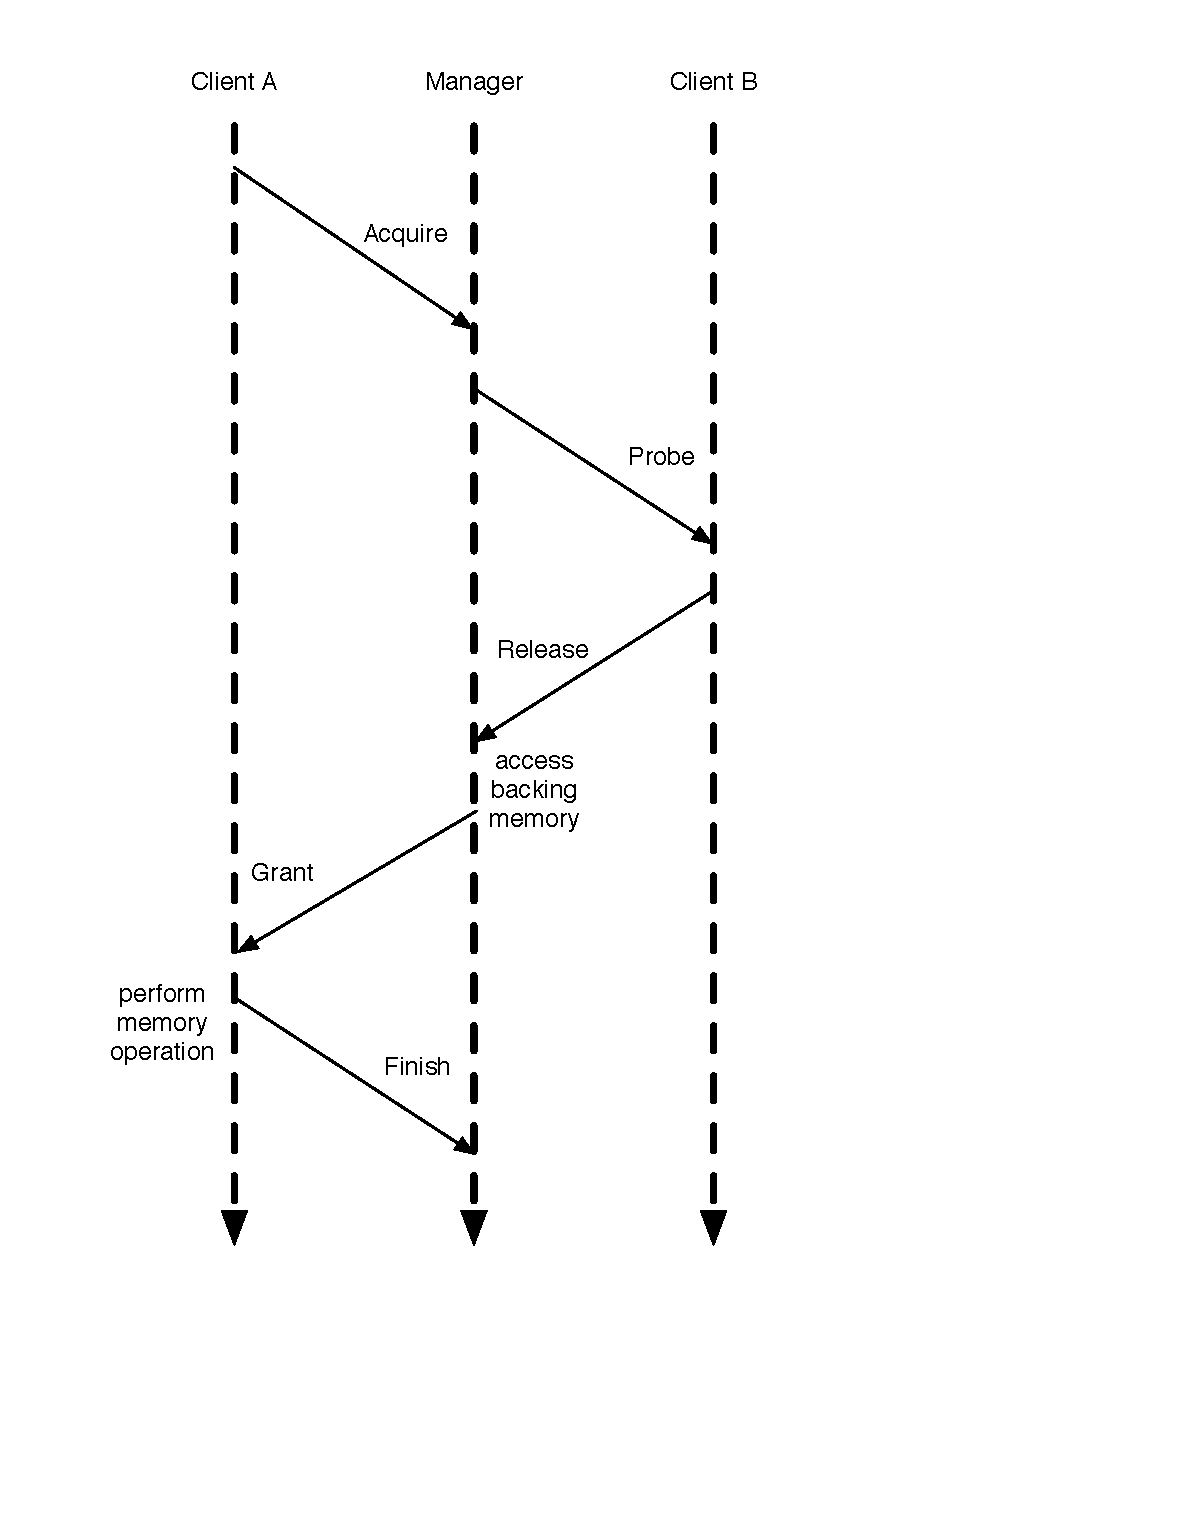
\includegraphics[width=0.6\columnwidth]{tilelink/figures/standard3.pdf}
\caption[Transaction flow to Acquire permissions on a cache block.]{
Overview of the transaction flow whereby a client acquires permissions on a cache block.
A client sends an Acquire to a manager.
The manager sends any necessary Probes to other clients.
The manager waits to receive a Release for every Probe that was sent.
The manager communicates with backing memory if required.
Having obtained the required data or permissions, the manager responds to the original requestor with a Grant.
Upon receiving a Grant, the original client responds to the manager with a Finish to complete the transaction.
}
\label{fig:standard3}
\end{figure}

There are two fundamental templates of transactions that can occur on a cache block managed by TileLink.
The first flow enables clients to acquire permissions to read or write data in a cache block.
Figure~\ref{fig:standard3} shows the message flow for this transaction in more detail.
After this transaction has completed, the client has acquired permissions to either read or write the cache block, as well as a copy of the block's data.
Other clients may have had to release their permissions on the block and write back dirty data in their possession.
If the manager is capable of tracking which clients have copies of the block using a directory, this metadata has been updated.

\begin{figure}[t!]
\centering
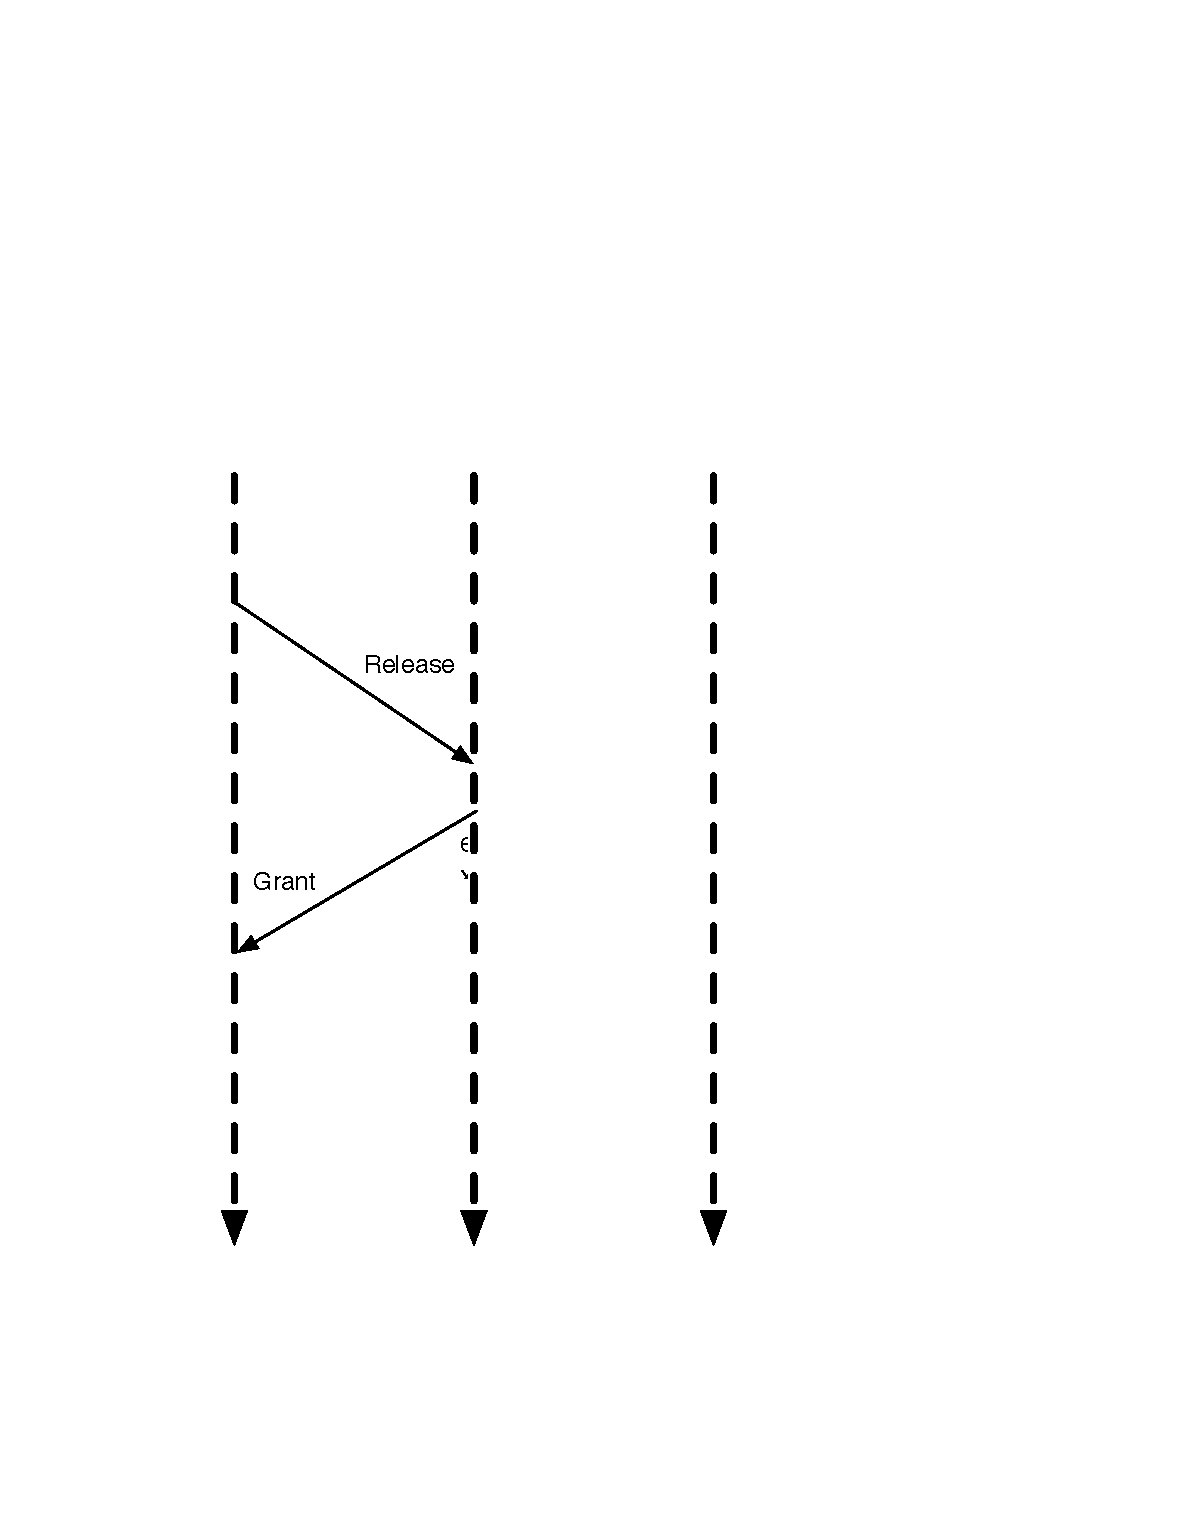
\includegraphics[width=0.5\columnwidth]{tilelink/figures/volwb.pdf}
\caption[Transaction flow to Release permissions on a cache block.]{
Overview of the transaction flow whereby a client voluntarily releases permissions on a cache block,
typically due to evicting the line for capacity reasons.
A client sends a Release to a manager, specifying that it is voluntary.
The manager communicates with backing memory if required.
The manager acknowledges completion of the transaction using a Grant.
}
\label{fig:volwb}
\end{figure}

The second type of transaction allows clients to voluntarily release their permissions on a cache block.
Figure~\ref{fig:volwb} shows the message flow for this transaction in more detail.
Typically, this type of transaction occurs when a cache must evict a block that contains dirty data, in order to replace it
with another block being refilled into the cache.
It might also be triggered by software hints, as we will discuss in Chapter~\ref{c.coherence}.
After this transaction has completed, the client has lost permissions to read or write the cache block, as well as its copy of the data.
If the manager is capable of tracking which clients have copies of the block using a directory, this metadata has been updated.

While these two flows form the basis of all TileLink transactions, there are a number of edge cases that arise when
they are overlaid on each other temporally or composed hierarchically.
The following sections discuss how responsibility for managing this complexity is distributed across the different TileLink agents.

\subsection{Concurrency in TileLink}

TileLink does not make any assumptions about the ordering of messages sent point-to-point over particular channels.
Therefore, concurrency must be managed by agents at several points in the system.
Imposing restrictions on agent behavior makes it possible for us to guarantee that a total ordering of transactions can be constructed,
despite the distributed nature of the problem and the lack of a global point of communication synchronization.
At the same time, we want to allow as much concurrency as possible among transactions whenever it is safe to do so.
There are three fundamental responsibilities to limit concurrency placed on TileLink agents:
\begin{itemize}
\item A manager should not accept another request for a transaction on a block that is already in-flight (unless it knows how to merge the two transactions as discussed below). Specifically, the manager must wait until it has received a Finish from the original client in order to ensure proper ordering of any future Grants on the same block to the same client.
\item If client has an outstanding voluntary writeback transaction, it cannot respond to an incoming Probe request on that block with Releases until it receives a Grant from the manager acknowledging completion of the writeback. It also cannot issue an Acquire on that block until it receives such a Grant.
\item If a client has an outstanding Acquire transaction, it should not issue further Acquires on that block unless they are of different types (for ``cached'' transactions)
or target different sub-block addresses (for ``uncached'' transactions). See Section~\ref{s.uncached} for details.
\end{itemize}

\begin{figure}[p]
\centering
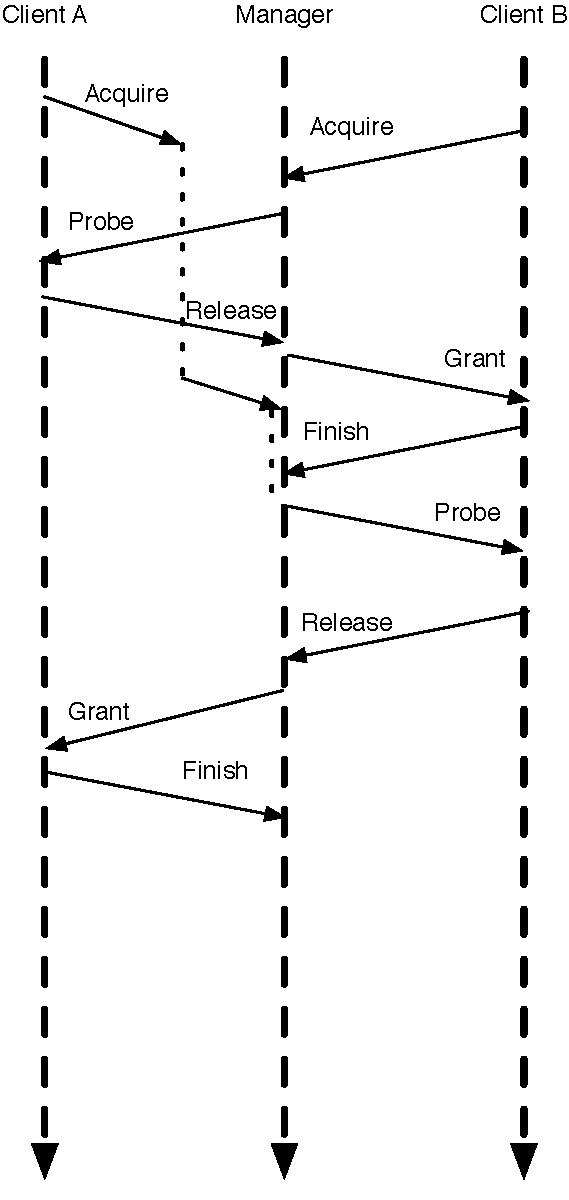
\includegraphics[width=0.5\columnwidth]{tilelink/figures/ordered.pdf}
\caption[Interleaved message flows demonstrating Manager blocking Acquires from multiple sources.]{
Interleaved message flows demonstrating Manager blocking Acquires from multiple sources.
Clients A and B send an Acquire to a Manager, with Client B winning the race.
The manager blocks Client A's transaction from making forward progress.
Client A must process any Probes issues by Client B's transaction, even though Client A has an Acquire outstanding.
The manager must respond with the correct type of Grant (including a copy of the data), given that Client A has been Probed since sending its Acquire.
Once Client B responds with a Finish, Client A's transaction can proceed as normal.
}
\label{fig:ordered}
\end{figure}

\begin{figure}[!p]
\centering
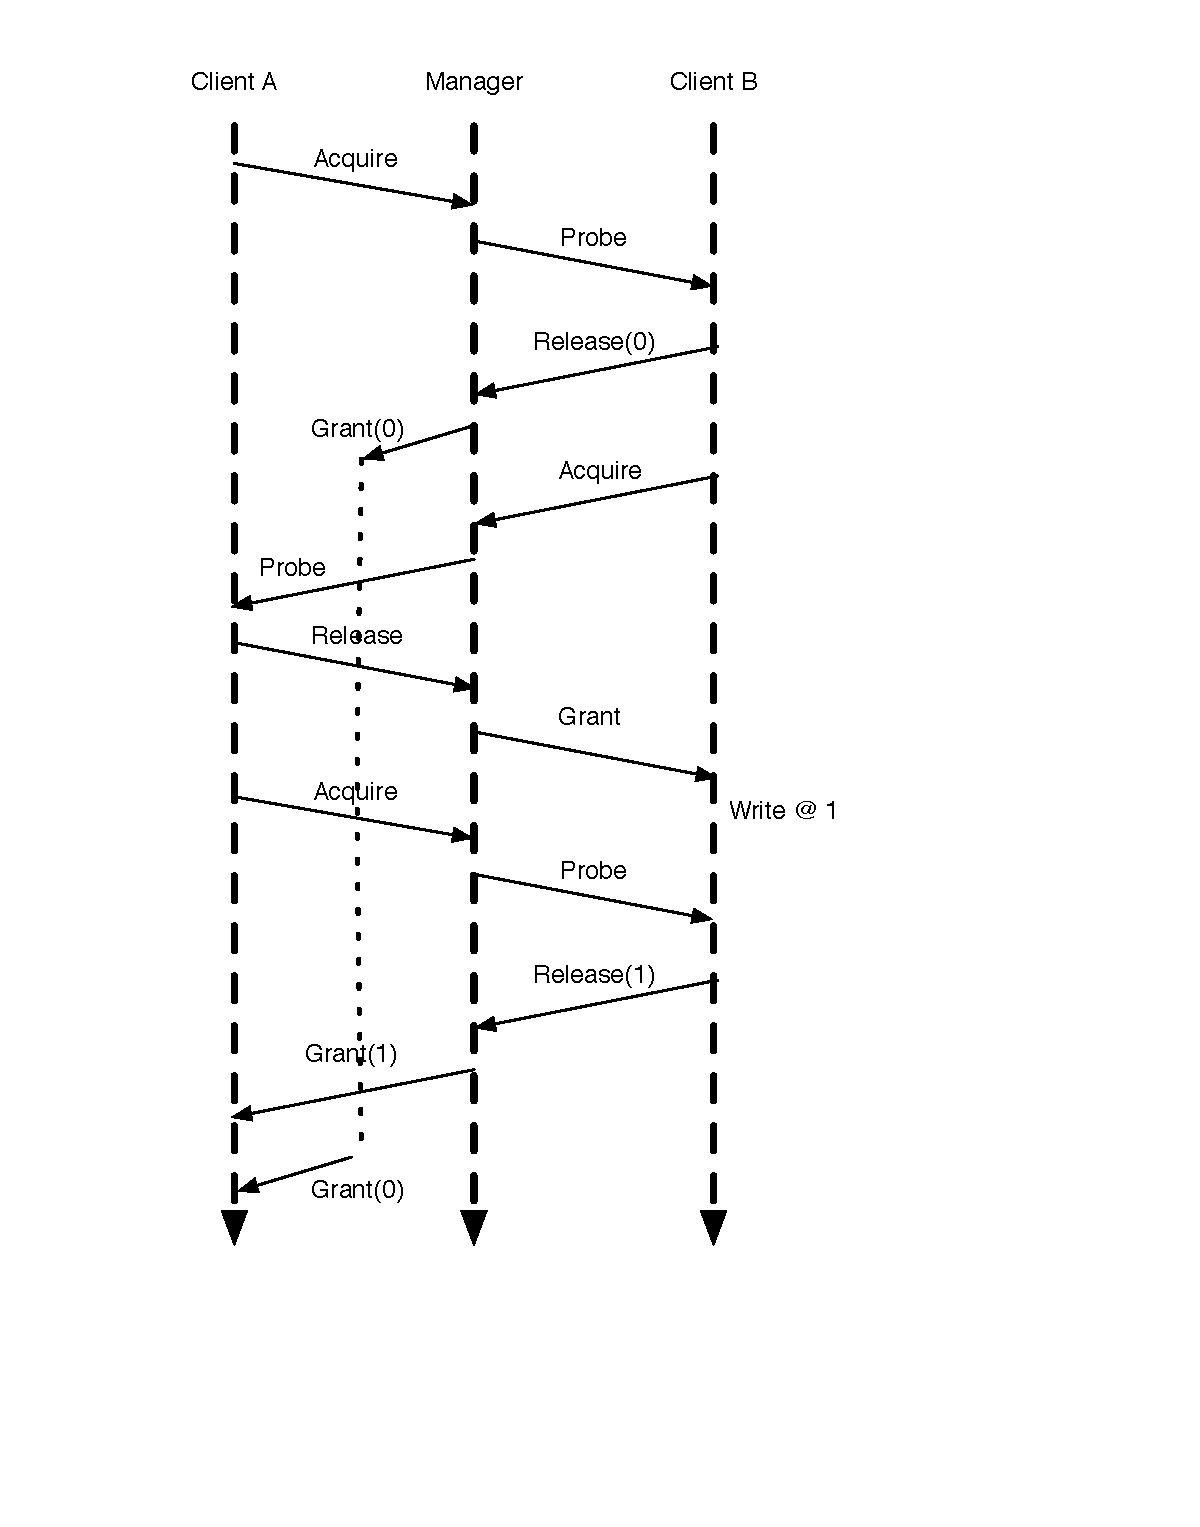
\includegraphics[width=0.5\columnwidth]{tilelink/figures/unordered.pdf}
\caption[Interleaved message flows demonstrating the need for Finishes to serialize Grant ordering.]{
Interleaved message flows demonstrating the need for Finishes to serialize Grant ordering.
Client A sends an Acquire to a manager, which in turn Probes Client B to Release dirty data.
This dirty data is forwarded by the manager in the form of a Grant to the transaction source, Client A.
Unfortunately, this Grant becomes delayed arbitrarily long in the unordered channel. 
Meanwhile, Client B initiates a transaction on the same block, Acquiring it in order to perform a write.
Client A must respond to the resultant Probe, even though it is still waiting for the missing Grant.
Client B is Granted permission to perform the write.
Client A then initiates a second transaction on the block, perhaps to upgrade its permissions, even though it is still waiting for the missing Grant.
Client B Releases the modified data, and it is Granted to Client A.
The second Grant bypasses the first Grant, and when the second Grant arrives, it overwrites the modified data with the original data.
Thus, from the perspective of Client A, the write to the block performed by Client B is lost.
}
\label{fig:unordered}
\end{figure}

\begin{figure}[!p]
\centering
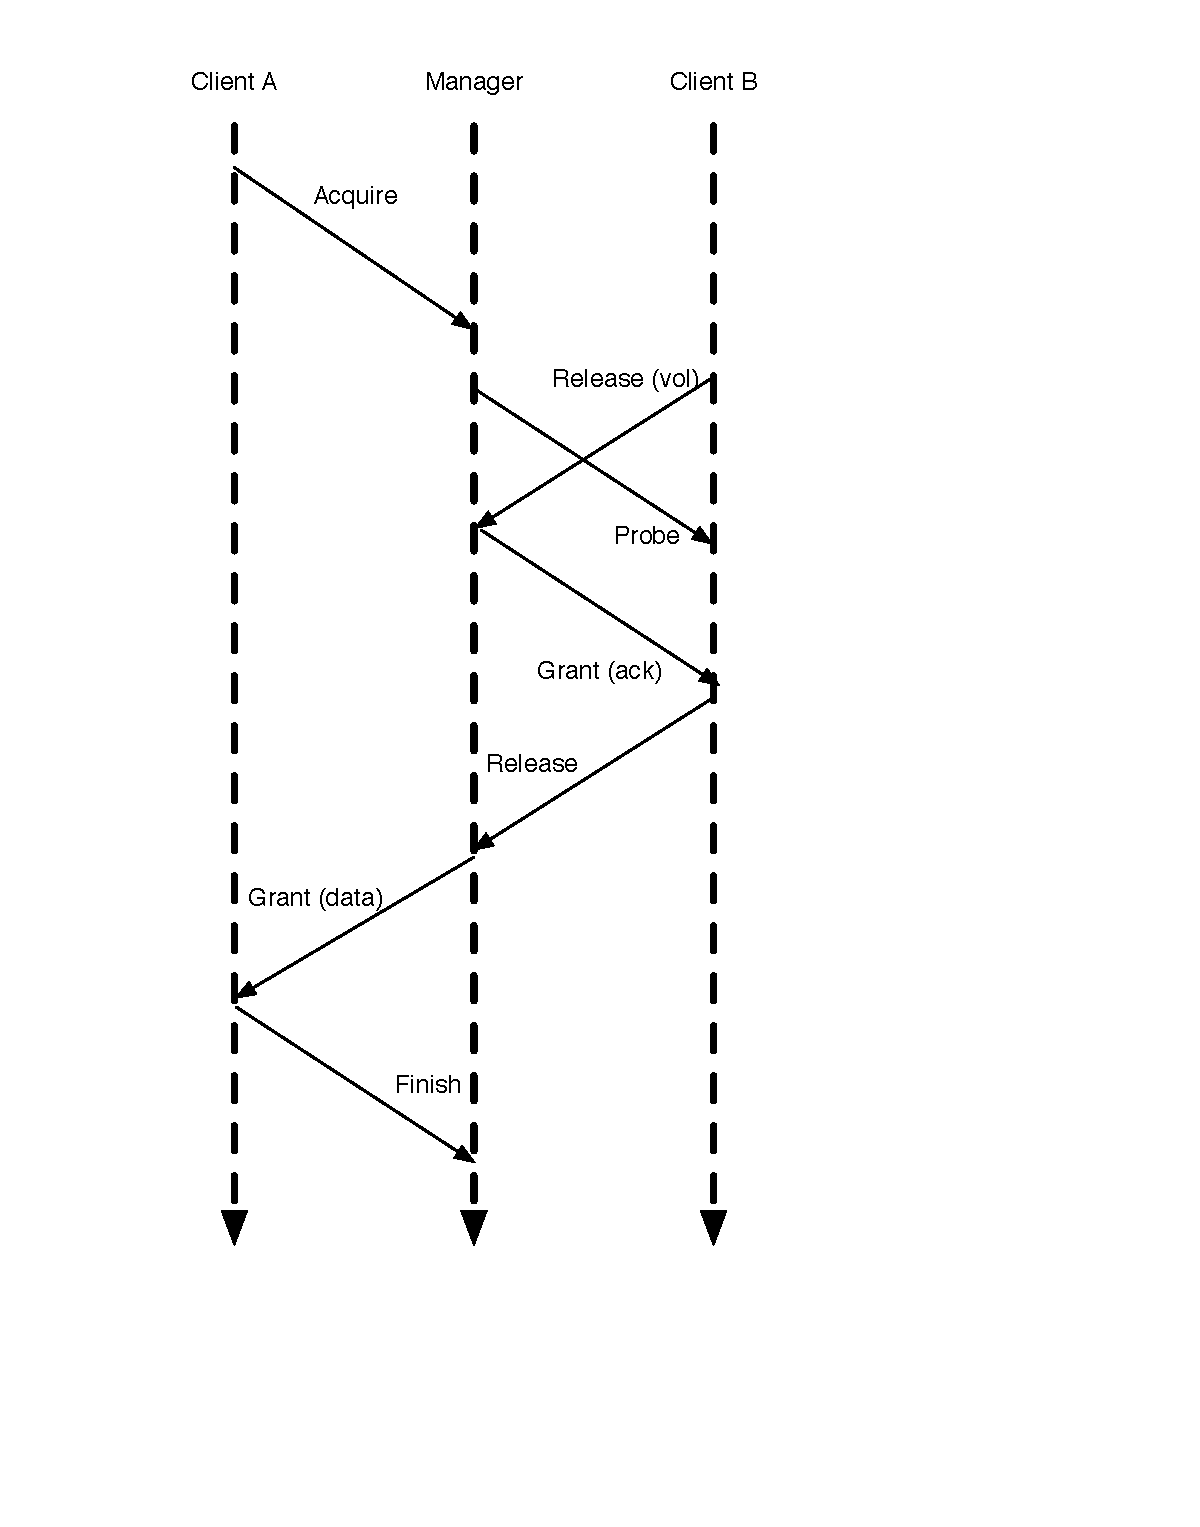
\includegraphics[width=0.5\columnwidth]{tilelink/figures/rel-merge.pdf}
\caption[Interleaved message flows demonstrating acknowledgment Grants of voluntary writeback Releases.]{
Interleaved message flows demonstrating acknowledgment Grants of voluntary writeback Releases.
Client A sends an Acquire to a manager, which then sends a Probe to Client B.
At the same time, Client B chooses to evict the same block and issues a voluntary Release.
The manager waits to receive a Release for every Probe that was sent, but additionally first accepts the voluntary Release.
The manager sends a special Grant that acknowledges receipt of the voluntary release.
Client B does not respond to the Probe until it gets the acknowledgment Grant.
Once Client B responds with a Release, Client A's transaction can proceed as normal.
}
\label{fig:rel-merge}
\end{figure}

We will first discuss the concurreny-limiting responsibility put on the manager.
The manager serves as a convenient point of synchronization across all the clients.
Since every transaction must be initiated via an Acquire message sent to a manager, the manager can trivially order the transactions.
A very safe implementation would be to accept only a single transaction's Acquire on a given cache block at a time,
but the performance implications of doing so are potentially dire, and it turns out we can be much more relaxed while continuing to provide a correct serialization.
Chapter~\ref{c:coherence} will provide an evaluation of the performance overheads of more limited TileLink concurrency.

At this time, TileLink forbids managers from accepting Acquires on the same cache block from different client sources.
Figure~\ref{fig:ordered} lays out this scenario in message sequence chart form.
Clients must continue to process and respond to Probes even with an outstanding Acquire pending in the network.
Managers must include an up-to-date copy of the data in Grants responding to Acquires upgrading permissions unless they are certain that that
client has not been Probed since the Aquire was issued.
Multiple acquires from the same source may be accepted, which we will discuss in more detail at the end of this section.
Assuming a manager has blocked on processing a second transaction Acquiring the same block, the critical question becomes: When is it safe for a manager to accept the pending Acquire?

If we were to assume point-to-point ordered delivery of messages over a particular channel,
it would be sufficient for the manager merely to have sent the Grant message to the original client source.
The manager could process further transactions on the block, and further Grants to the same client would arrive in order.
The act of updating the block's metadata and sending the Grant message is sufficient to serialize the transaction in the total ordering of transactions on the block.

However, TileLink intentionally does not make the point-to-point ordered delivery assumption.
Grants on the same block sent to the same client can arrive out of order.
Figure~\ref{fig:unordered} lays out this scenario in message sequence chart form.
Because Grants can arrive out of order, TileLink requires the addition of a final acknowledgment channel (Finish), which ensures that each Grant has been received by the client.
Note that some prior coherence protocols have addressed this particular complexity by blocking Probes until the Grant gets back to the source, but we will discuss why this solution can
cause deadlick in a hierarchical, nested system in the next section.

We now turn to the second concurrency-limiting responsibility, which is put on the client.
If a client has an outstanding voluntary writeback transaction on a block,
it cannot respond to an incoming Probe request on that block with Releases until it receives a Grant from the manager acknowledging completion of the writeback.
This limitation serializes the ordering of the voluntary writeback relative to the ongoing Acquire transaction.
The manager cannot simply block the voluntary release transaction until the Acquire transaction completes, because the Release message in that transaction will be
blocked behind the voluntary Release.
Figure~\ref{fig:rel-merge} lays out this scenario in message sequence chart form.

From the manager agent's perspective, it must handle the situation of receiving a voluntary Release for a block which another client is currently attempting to Acquire.
The manager must accept the voluntary Release as well as any Releases resulting from any Probe messages that have already been sent, and afterwards provide Grant messages to both clients before the transaction can be considered complete.
The voluntary write's data can be used to respond to the original requestor with a Grant, but the transaction cannot complete until the expected number of Releases
have been collected by the manager.
This scenario is an example of two transaction message flows being merged by the manager agent.

The final concurrency-limiting responsibility put on the client agent is to issue multiple Acquires for the same block only when the transactions can be differentiated from one another.
Typically, this differentiation takes the form of having different Acquire types or different transaction identifiers.
One possible case is for a client that has a write miss under a read miss to issue an Acquire asking for write permission before the Grant providing read permissions has arrived.
Managers are not obligated to accept both Acquires and merge the transactions' message flows, though they may choose to do so.
Further restrictions on issuing multiple Acquires to sub-block addresses via built-in transactions are detailed in Section~\ref{s.uncached}.


\subsection{Hierarchical TileLink}
\label{s.tlhier}

\begin{figure}[p]
\centering
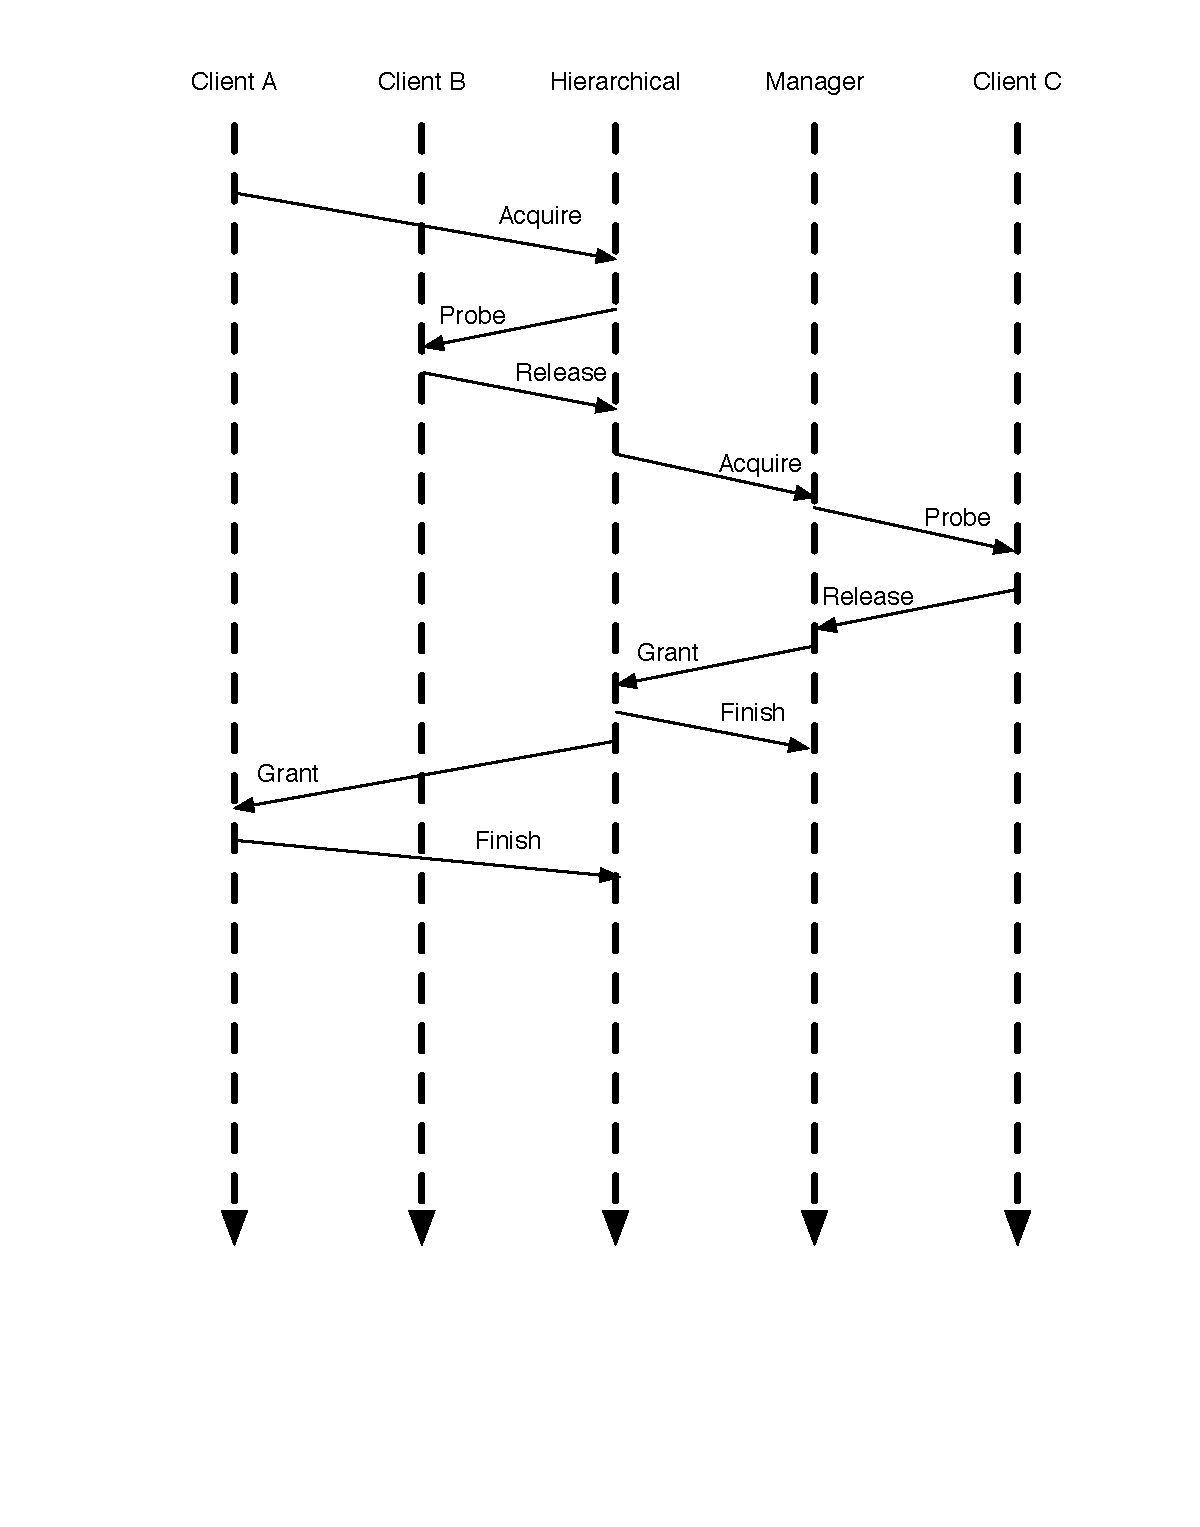
\includegraphics[width=0.8\columnwidth]{tilelink/figures/standard5.pdf}
\caption[Overview of a multi-level transaction's message flow.]{
Overview of a multi-level transaction's message flow.
After the hierarchical agent has Probed the clients under its purvue, it falls back on initiating a transaction in the outer realm,
which is serviced by the outermost manager. Other branches of the memory hierarchy are Probed,
and any Released data is Granted back to the original source Client A by way of the hierarchical agent.
}
\label{fig:standard5}
\end{figure}

\begin{figure}[!p]
\centering
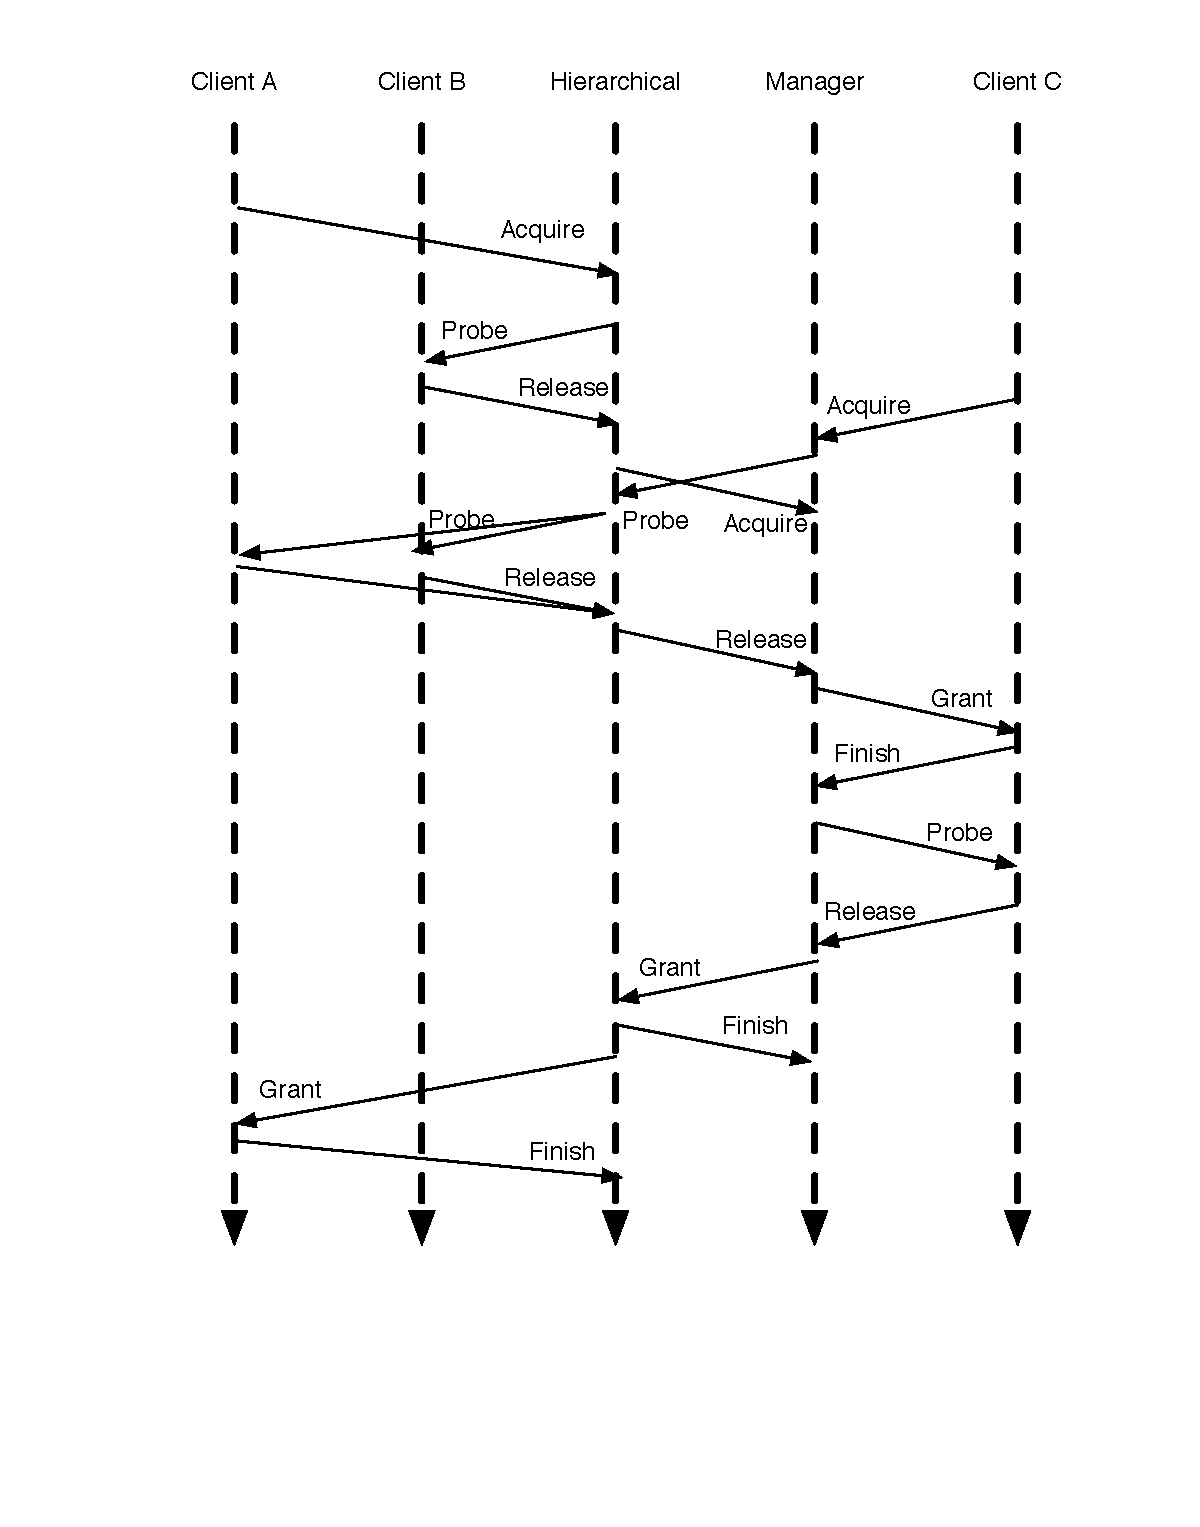
\includegraphics[width=0.8\columnwidth]{tilelink/figures/acq-merge-5.pdf}
\caption[Overview of a multi-level transaction's message flow including an Acquire race.]{
Overview of a multi-level transaction's message flow including an Acquire race.
Client A and Client C both issue Acquires. However, Client C's Acquire is the first to reach the outermost Manager, which means
it happens before Client A's transaction.
Client A must deal with Probes generated as part of Client C's transaction without deadlocking, even though it has already sent its own Acquire.
The Grant sent by the Hierarchical agent must take into account the fact that Client A was Probed mid-transaction.
}
\label{fig:acq-merge-5}
\end{figure}

\begin{figure}[!p]
\centering
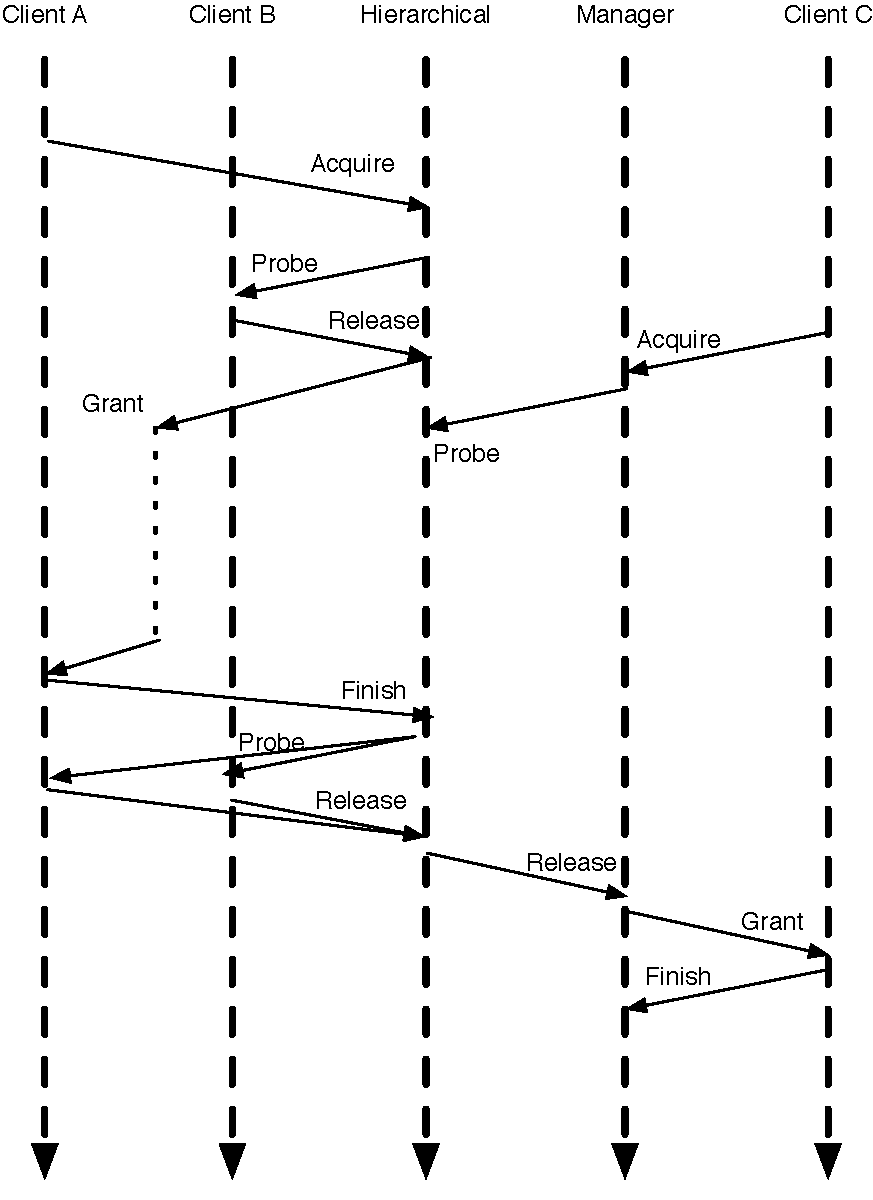
\includegraphics[width=0.8\columnwidth]{tilelink/figures/acq-merge-5-2.pdf}
\caption[Overview of a multi-level transaction's message flow including an Acquire race.]{
Overview of a multi-level transaction's message flow including an Acquire race.
Client A and Client C both issue Acquires.
Client A's transaction is satisfiable locally, and a Grant is issued for it, which becomes delayed in the network.
Client C's Acquire is the first and only to reach the outermost Manager.
Client A must deal with Probes generated as part of Client C's transaction without deadlocking, even though it has already sent its own Acquire
and the Hierarchical agent has issued a Grant in response.
The Hierarchical Agent must wait until the Grant's Finish is received before forwarding the outer Probes inward.
}
\label{fig:acq-merge-5-2}
\end{figure}

TileLink is a hierarchical protocol that ascribes to the Manager-Client Pairing (MCP) architecture.
Each manager tracks and serializes transactions for all the clients within its coherence realm.
In situations where a manager does not have access or permissions on a particular piece of data,
it will in turn initiate a transaction in an outer realm.
Memory controllers at the root of the memory hierarchy are the ultimate managers, and they always have permission
to supply the data in the address range they control.

This structure results in nested sequences of messages, and we discuss some of the concurrency edge cases for these message flows here.
Details of how a transaction initiated in an inner realm is translated into the protocol of the outer realm are left to the next chapter.
Figure~\ref{fig:standard5} lays out a basic multi-level transaction in message sequence chart form.
The transaction between the hierarchical agent and the outermost manager is nested within the inner transaction.
The outer Acquire is sent based on the inner Acquire. 
The inner Grant is dependent on the outer Grant response.
Probes may be launched into other branches of the memory hierarchy.

Figures~\ref{fig:acq-merge-5}~and~\ref{fig:acq-merge-5-2} lay out concurrency races between two multi-level transactions in message sequence chart form.
The transaction whose Acquire is first to reach the outermost Manager required to gain sufficient permissions happens before the other transaction,
and the final state of the data and permissions in the system must reflect this ordering.
The transaction that won the race in the outer level may issue Probes into the branch of the memory hierarchy where the other transaction has begun to be processed.
These Probes must be responded to with Releases to prevent deadlock in the outer level.
However, this means that the inner transaction and outer transaction must be merged successfully.
If the inner transaction has not yet sent a Grant to the originator (Figure~\ref{fig:acq-merge-5}),
the Grant sent must take into account the fact that Client A was Probed mid-transaction.
If the inner transaction has already sent a Grant to the originator (Figure~\ref{fig:acq-merge-5-2}),
then the outer Probes must not be forwarded until the receipt of the Grant is acknowledged with a Finish message from the original client.

\section{Built-in Transactions}
\label{s.uncached}

One of the design goals of TileLink was to support heterogeneous SoC designs that consist of a wide variety of agents.
In particular, we wanted to support accelerators that operate on the same global shared memory space as the general-purpose cores, possibly at very high bandwidths.
However, while these accelerators need a coherent view of memory, they do not necessarily cache copies of data themselves.
We wanted cacheless accerators to be able to interoperate with any coherence policy implemented on top of the TileLink protocol, without having to know anything about coherence policies internally.

These design goals led us to create a set of {\em built-in} transactions available to any client connected to a TileLink substrate.
We provide seven built-in transaction types that are available to all clients that want to participate in the coherence protocol, even if they themselves will not keep cached copies of the data.
Because these transactions do not create a new private copy of the targeted cache block, we term them ``uncached'' transactions. 
However, they still participate in the standard TileLink transaction flow, meaning that they will result in probes of other caches and return coherent answers.

\subsection{Built-in Transaction Types}

The uncached transactions available to all TileLink clients are as follows:
\begin{description}
\item[Get:] Fetches a single beat of data from a cache block and returns only that beat.
\item[GetBlock:] Fetches an entire cache block and serves it back to the requestor.
\item[GetPrefetch:]  Prefetches a cache block into the next-outermost level of the memory hierarchy with read permissions.
\item[Put:] Writes up to a beat's worth of data to backing memory. Uses a write mask to determine which bytes contain valid write data.
\item[PutBlock:] Writes out an entire cache block to backing memory.
\item[PutPrefetch:]  Prefetches a cache block into the next-outermost level of the memory hierarchy with write permissions.
\item[PutAtomic:] Performs an atomic memory op in the next-outermost level of the memory hierarchy. The maximum available operand size is 64b (sizes and opcodes per RISC-V atomic instructions).
\end{description}

There are five built-in types of Grant that are available to all managers that want to participate in the coherence protocol.
Because ``uncached'' transactions do not create a new private copy of the targeted cache block, we use these Grant types mostly as acknowledgments.
The available types are as follows:
\begin{description}
\item[GetDataBlock:] Full cache block in response to Acquire.GetBlock.
\item[GetDataBeat:] Single beat of data in response to Acquire.Get or Acquire.PutAtomic.
\item[PutAck:] Acknowledgement of Acquire.\{Put, PutBlock\}.
\item[PrefetchAck:] Acknowledgment of Acquire.\{GetPrefetch, PutPrefetch\}.
\item[VoluntaryAck:] Acknowledgement of any voluntary Release.
\end{description}

The PutBlock message is unique among the built-in Acquire types in that it contains multiple beats of data (if the cache block size is larger than the parameter {\tt TLDataBits}).
The client controller that generates this message is responsible for generating multiple sequential PutBlock messages and incrementing the {\tt addr\_beat} field as it does so.
The GetDataBlock message also contains multiple beats of data (again, if the cache block size is larger than {\tt TLDataBits}).
The manager controller that generates this message is responsible for generating multiple sequential GetDataBlockmessages and incrementing the {\tt addr\_beat} field as it does so.
In contrast, a GetDataBeat message only ever consists of a single beat.
A single VoluntaryAck is used to respond to each voluntary Release, even if that Release consists of multiple beats.
Similarly, a single PutAck is used to respond to a PutBlock message containing multiple beats.

\begin{table}[ht]
\begin{center}
\begin{tabular}{|l|l|l|}
    \hline
    Acquire & Grant & Effect \\ \hline \hline
    Get & GetDataBeat & Copy data in to client \\ \hline
    GetBlock & GetDataBlock & Copy data in to client \\ \hline
    GetPrefetch & PrefetchAck & Fetch data to outer memory with read permissions \\ \hline
    Put & PutAck & Update data in outer memory \\ \hline
    PutBlock & PutAck & Update data in outer memory \\ \hline
    PutPrefetch & PrefetchAck & Fetch data to outer memory with write permissions \\ \hline
    PutAtomic & GetDataBeat & Update data in outer memory and return old value. \\ \hline
\end{tabular}
\end{center}
\caption{Overview of built-in, uncached transactions. Each type of Acquire results in a particular acknowledgment or data Grant.}
\label{tab:uncached}
\end{table}

Table~\ref{tab:uncached} provides and overview of the built-in transactions and their effect on memory.
In a hierarchical system, uncached transactions may be turned into cached transactions in outer levels of the memory hierarchy.
We provide an allocation flag on the Acquire messages to govern whether this conversion is allowed.

Whether an address is cached or uncached is a property of the transaction, not the address. Certain clients may cache an address, while other clients at the same level may not. If the allocation flag is set to true, a hierarchical agent may choose to convert an uncached transaction into a cached one, which will result in the data becoming cached at the outer level. It will still not be cached by the original requestor (who asked for it uncached). If the allocation flag is false, the hierarchical agent must also issue the transaction uncached and merely forward the grant back to the original requestor without caching the data locally.
 
\subsection{Memory Model for Built-In Sub-Block Transactions}

TileLink is intended to be compatible with the weak memory consistency model adopted by the RISC-V ISA, but it should be compatible with any similarly weak model.
TileLink channels are not required to perform in-order delivery of messages, and hierarchical and manager agents are not required to process transactions in a particular order.
Therefore, client agents are responsible for enforcing orderings between memory operations by
waiting to initiate new transactions until all relevant outstanding transactions have been completed.
Uncached transactions that do not return data to the client still receive acknowledgments of operation completion from the manager, which allows for clients to make decisions about when to issue further requests.
It is worth noting that clients should always avoid issuing multiple requests to any particular address at the same time, as the Acquire messages may be reordered, resulting in non-sequential memory operation orderings.

\subsection{Concurrency for Built-In Sub-Block Transactions}

\begin{figure}[p]
\centering
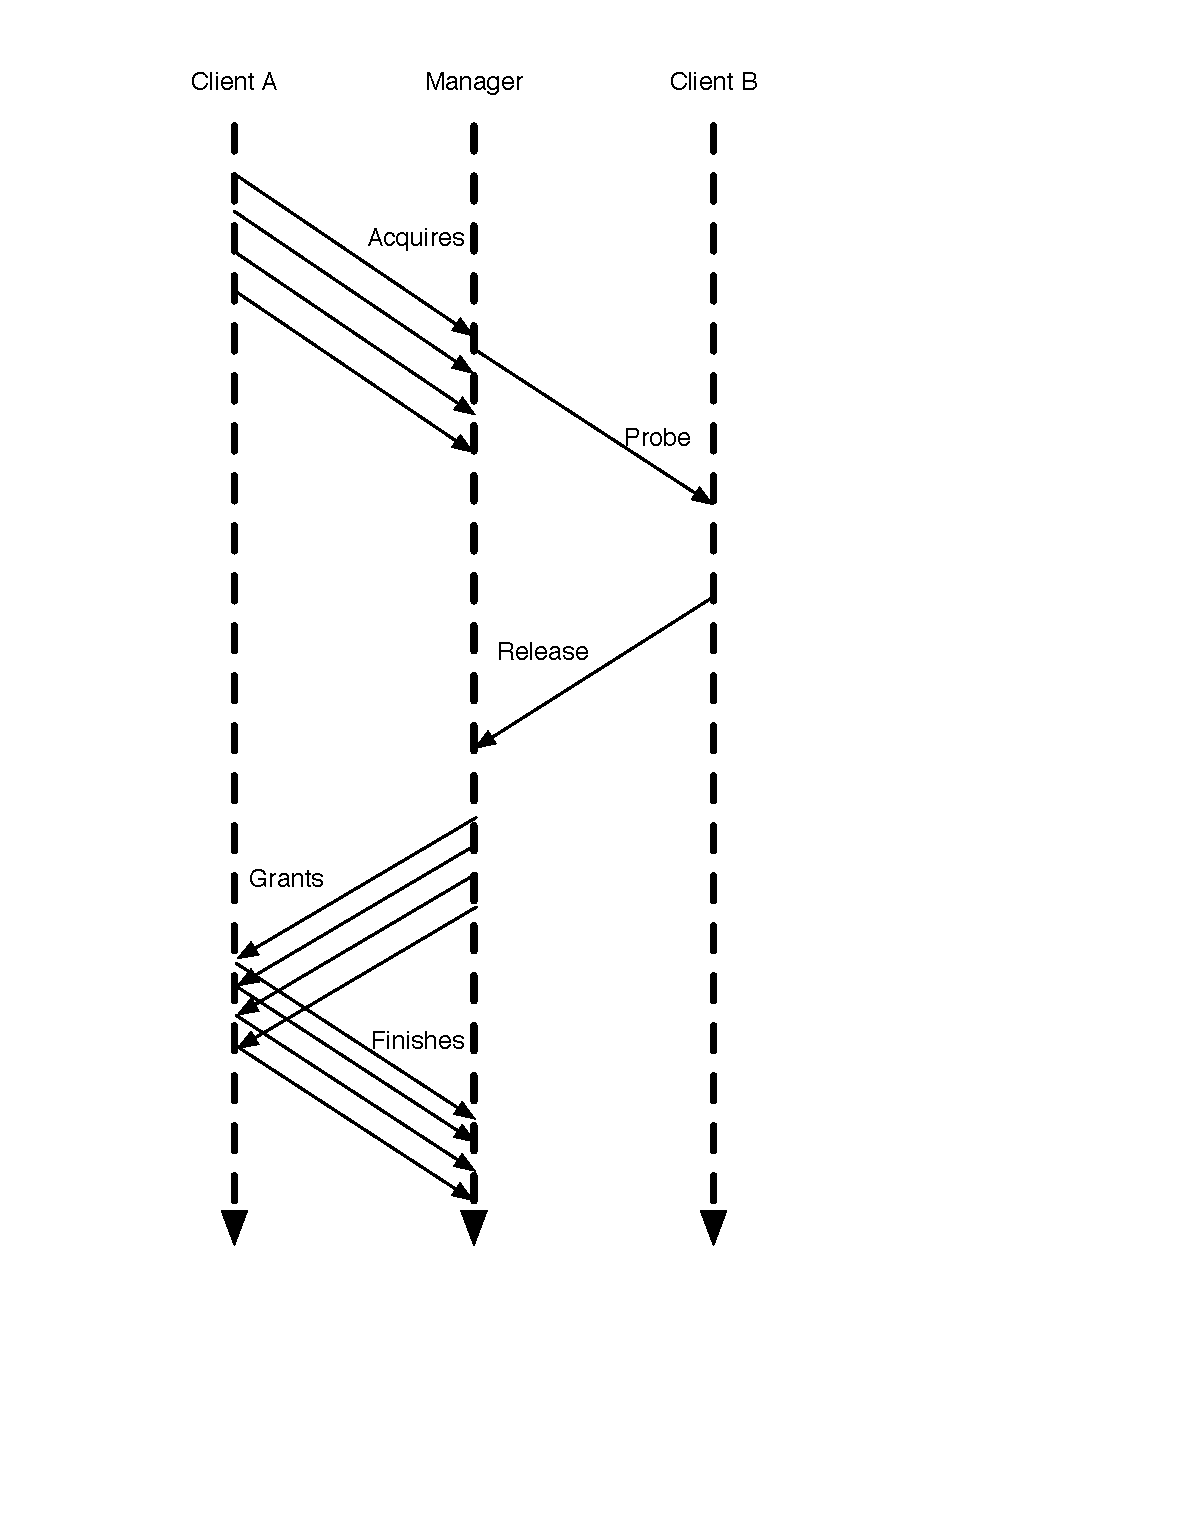
\includegraphics[width=0.5\columnwidth]{tilelink/figures/acq-merge.pdf}
\caption[Interleaved message flows merging of multiple ``uncached'' transactions.]{
Interleaved message flows demonstrating merging of multiple ``uncached'' transactions from the same client.
As long as the Acquires target different sub-block addresses they are safe to interleave.
Multiple Grants and Finishes can also be in flight simultaneously, and the transaction terminates when the correct count of Finishes is accepted.}
\label{fig:acq-merge}
\end{figure}

In order to support high-bandwidth access to cached data blocks from data-parallel accelerators, TileLink enables many outstanding built-in, sub-block transactions
to be in flight in the memory hierarchy at once.
In general, it is preferable to merge such transactions on the client side, before they are even exposed to the TileLink interface.
However, in order to provide support for secondary misses in hierarchical agents, we define the following rules for transaction merging.

As long as the Acquires used to initiate the transaction target different sub-block addresses, it is safe to interleave their processing by merging the transactions with one another.
The Acquires must be attempting to gain the same permissions and perform the same operation.
They must also have unique transaction identifiers.
Acquires from multiple client agents can be merged so long as they meet the above requirements.

Figure~\ref{fig:acq-merge} illustrates a merging scenario from a single client.
Multiple Grants and Finishes can also be in flight simultaneously, and the overall merged transaction terminates when the correct count of Finishes is accepted.
In order to prevent starvation of other clients, merging secondary sub-block transactions should not be prioritized over processing transactions initiated by other clients.
Merging transactions is an allowable performance optimization, not a requirement.

\section{Assumptions and Guarantees}

As we move towards a formal specification of TileLink, an important step is to provide a set of invariants to which any implementation must conform.
If any of these assumptions are not met by a particular implementation of physical network, client agent,
or manager agent, then the system can either deadlock or produce an incoherent view of global shared memory.
Conversely, composing a set of implementations that meet all these assumptions will
guarantee a deadlock-free implementation of cache coherency.
The following list collects the requirements necessary for a correct TileLink implementation:
\begin{itemize}
\item If a message contains multiple beats of data, all beats will eventually be sent.
\item A client issuing an Acquire will eventually receive a corresponding Grant.
\item A client receiving a Grant will issue a corresponding Finish,
unless the physical network is known to provide in-order delivery.
\item A client receiving a Probe will issue a corresponding Release.
\item A client issuing a voluntary Release will receive a corresponding Grant (of type VoluntaryAck), 
unless the physical network is known to provide in-order delivery.
\item Managers always consume any available Finish messages.
\item No duplicate messages will be created by any agents or within any channels.
\item All messages will eventually be delivered by the physical channels; a message cannot be lost.
\item No Finish is ever blocked by another message type.
\item Grants may only be blocked by Finishes.
\item Releases may only be blocked by Finishes and Grants.
\item Probes may only be blocked by Finishes, Grants, and Releases.
\item If a client has an outstanding voluntary Release on a block, it will not respond to a Probe on that block until it receives the Release's corresponding Grant.VoluntaryAck.
\item If a client has an outstanding voluntary Release on a block, it will not issue an Acquire on that block until it receives the Release's corresponding Grant.VoluntaryAck.
\item If a manager has already has accepted an Acquire on a block, it will not issue Probes or Grants in response to a second Acquire on that block until it recieces a Finish from the first Acquire's source.
\item A manager will always include a copy of the data in a Grant, unless it can prove that the client had a copy of the block when the Acquire was accepted and no Probes from outer memory for that block have been received.
\item Clients may not issue multiple Acquires with the same {\tt client\_xact\_id} and {\tt addr\_block} fields, unless they have different {addr\_beat}, {a\_type}, or {union} fields.
\item In a multi-level system, the transaction whose Acquire is first to reach the outermost Manager required to gain sufficient permissions happens before the other transaction.
The final state of the data and permissions in the system must reflect this ordering.
\item A Hierarchical agent will block Probes from being forwarded from its outer client interface to its inner manager interface until it has received Finishes for all Grants on that block.
\end{itemize}

\section{Channel Signal Descriptions}
\label{s.types}

This section details the specific signals contained in each channel of the TileLink protocol.
Every channel is wrapped in a decoupled interface, meaning that each contains ready and valid signals as well as the following bundles of signals.
Channels whose message types may contain data (i.e., Acquires, Releases and Grants) may send the data over multiple beats
if the cache block size is larger than \code{TLDataBits}.
The agent controller that generates these multi-beat messages is responsible for generating the correct number of sequential beat messages and incrementing the \code{addr\_beat} field as it does so.
Tracking beat counts in this way exposes the width of the underlying network to the controllers, 
but we propose that this encapsulation deficiency is necessary in order to improve the efficiency of refilling data into caches whose data array rows are of a matching size to the physical network.


%\subsection{Acquire}

\emph{Acquires} initiate a transaction to acquire access to a cache block with proper permissions for a particular memory operation.
Acquires are also used to write data into outer memory (acquiring permissions for the write as it does so), perform an atomic operation in outer memory, or prefetch data with particular permissions.
Table~\ref{tab:acquire} shows all the fields of the Acquire channel.
Some of the fields used for certain built-in transactions are multiplexed onto the Union field.
Table~\ref{tab:union} shows all these sub-fields and indicates which are used for each type
of built-in Acquire message.

\begin{table}[p]
\begin{center}
\begin{tabular}{|l|l|l|}
    \hline
    Name & Type & Purpose \\ \hline \hline
addr\_block & UInt & Physical address of the cache block, with block offset removed \\ \hline
client\_xact\_id & UInt & Client's id for the transaction \\ \hline
data & UInt & Client-sent data, used for Put transactions \\ \hline
addr\_beat & UInt & Offset of this beat's worth of data within the cache block \\ \hline
built\_in\_type & Bool & Whether the transaction is a built-in or custom type \\ \hline
a\_type & UInt & Type of the transaction. For built-in transactions, one of: \\
        &      & \{Get, GetBlock, GetPrefetch, Put, PutBlock, PutPrefetch, PutAtomic\}, \\
        &      &  Otherwise defined by the coherence protocol \\ \hline
union & Union & Used to derive and derive the sub-fields in Table~\ref{tab:union} \\ \hline
\end{tabular}
\end{center}
\caption{Fields of the Acquire channel.}
\label{tab:acquire}
\end{table}

\begin{table}[]
\begin{center}
\begin{tabular}{|l|l|c|c|c|c|l|}
    \hline
Name       & Type & Get & Put & Atomic & Prefetch & Purpose \\ \hline \hline
allocate   & Bool & X   & X   &        &          & Hints whether to allocate data in outer caches \\
           &      &     &     &        &          & when servicing this request \\ \hline
op\_code   & UInt & X   & X   & X      & X        & Memory op code; see Appendix~\ref{a.memopcodes}) \\ \hline
op\_size   & UInt &     &     & X      &          & Size of the AMO operands (b/h/w/d) \\ \hline
addr\_byte & UInt & X   &     & X      &          & Address of the word within the block \\ \hline
wmask      & UInt &     & X   &        &          & Byte write mask for Put data \\ \hline
\end{tabular}
\end{center}
\caption{Input sub-fields used to fill in the Union field of the Acquire channel for built-in messages.
`X' indicates which  subfields are meaningful for which built-in message types.
}
\label{tab:union}
\end{table}


%\subsection{Probe}

\emph{Probes} query a client to determine whether it has a cache block or to revoke that client's  permissions on that cache block.
Table~\ref{tab:probe} shows all the fields of the Probe channel.

\begin{table}[]
\begin{center}
\begin{tabular}{|l|l|l|}
    \hline
    Name & Type & Purpose \\ \hline \hline
addr\_block & UInt & Physical address of the cache block, with block offset removed \\ \hline
p\_type & UInt & Transaction type, defined by coherence protocol \\ \hline
\end{tabular}
\end{center}
\caption{Fields of the Probe channel.}
\label{tab:probe}
\end{table}


%\subsection{Release}

\emph{Releases} provide an acknowledgment of Probe receipt by clients, releasing certain permissions on the block along with any dirty data back to the manager.
Releases are also used by clients to voluntarily write back data or cede permissions on the block.
Table~\ref{tab:release} shows all the fields of the Release channel.

%Release messages may contain multiple beats of data (if the cache block size is larger than TLDataBits).
%The client controller that generates this message is responsible for generating multiple sequential Release messages and incrementing the \code{addr\_beat} field as it does so.

\begin{table}[]
\begin{center}
\begin{tabular}{|l|l|l|}
    \hline
    Name & Type & Purpose \\ \hline \hline
addr\_block & UInt & Physical address of the cache block, with block offset removed \\ \hline
client\_xact\_id & UInt & Client's id for the transaction \\ \hline
data & UInt & Used to writeback dirty data \\ \hline
addr\_beat & UInt & Offset of this beat's worth of data within the cache block \\ \hline
r\_type & UInt & Transaction type, defined by coherence protocol \\ \hline
voluntary & Bool & Whether this release is voluntary or in response to a Probe \\ \hline
\end{tabular}
\end{center}
\caption{Fields of the Release channel.}
\label{tab:release}
\end{table}

%\subsection{Grant}

\emph{Grants} provide data or permissions to the original requesting client, granting it access to the cache block.
Grants are also used to acknowledge voluntary Releases.
Table~\ref{tab:grant} shows all the fields of the Grant channel.

%The GetDataBlock message may contain multiple beats of data (if the cache block size is larger than TLDataBits).
%The manager controller that generates this message is responsible for generating multiple sequential
%GetDataBlock messages and incrementing the \code{addr\_beat} field as it does so.

\begin{table}[]
\begin{center}
\begin{tabular}{|l|l|l|}
    \hline
    Name & Type & Purpose \\ \hline \hline
built\_in\_type & Bool & Whether transaction type is built-in or custom \\ \hline
g\_type & UInt & Type of the transaction. For built-in transactions, one of: \\
        &      & \{VoluntaryAck, PrefetchAck, PutAck, GetDataBeat, GetDataBlock\}. \\
        &      & Otherwise defined by the coherence protocol \\ \hline
client\_xact\_id & UInt & Client's id for the transaction \\ \hline
manager\_xact\_id & UInt & Manager's id for the transaction, passed to Finish \\ \hline
data & UInt & Used to supply data to original requestor \\ \hline
addr\_beat & UInt & Offset of this beat's worth of data within the cache block \\ \hline
\end{tabular}
\end{center}
\caption{Fields of the Grant channel.}
\label{tab:grant}
\end{table}


%\subsection{Finish}

\emph{Finishes} provide a final acknowledgment of transaction completion from requestor and are used to preserve transaction ordering.
Table~\ref{tab:finish} shows all the fields of the Finish channel.

\begin{table}[]
\begin{center}
\begin{tabular}{|l|l|l|}
    \hline
    Name & Type & Purpose \\ \hline \hline
manager\_xact\_id & UInt & Manager's id for the transaction \\ \hline
\end{tabular}
\end{center}
\caption{Fields of the Finish channel.}
\label{tab:finish}
\end{table}

\section{Agent-Specific Views of Logical TileLink Networks}

\begin{figure}[p]
\centering
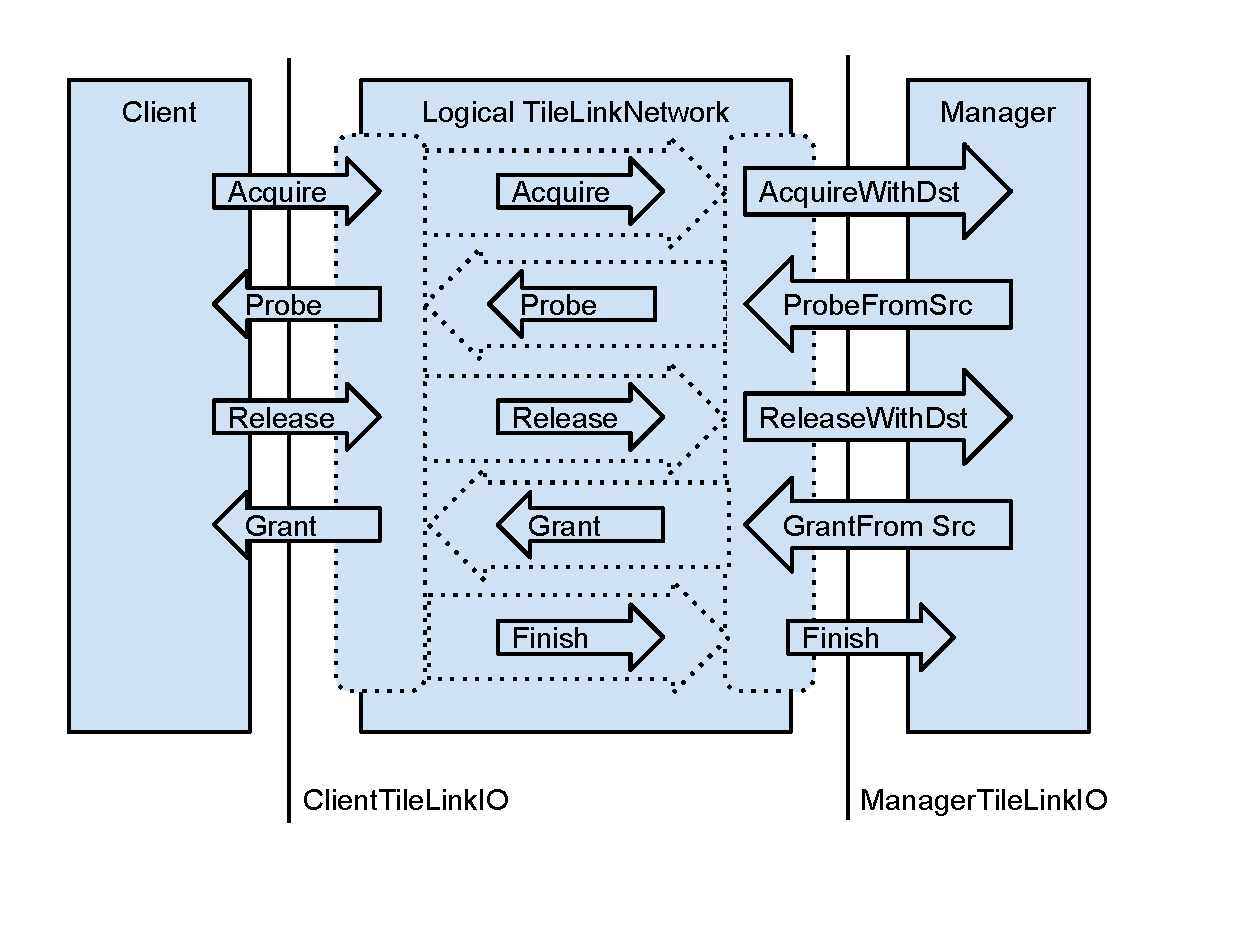
\includegraphics[width=1\columnwidth]{tilelink/figures/agent-specific.pdf}
\caption{Overview of the logic view of the TileLink interface presented to each type of agent.}
\label{fig:agent}
\end{figure}

For the convenience of designers implementing Client and Manager agents, we provide TileLinkNetworkPort modules which abstract away the details of the on-chip network implementation.
These network ports automatically generate networking headers, perform SerDes for narrower physical network channels, and generate appropriate control flow logic.
The ports then expose simplified subsets of the TileLink channels to the agent modules.
Figure~\ref{fig:agent} provides an overview of these two interfaces.

{\em ClientTileLinkIO} consists of standard Acquire, Probe, Release, and Grant message channels.
It does not include the Finish channel as generating those acknowledgments is handled by the ClientTileLinkNetworkPort.

{\em ManagerTileLinkIO} consists of Acquire, Probe, Release, and Grant message channels that have additional data appended about the source or destination of messages, expressed in terms of the Client's id.
Acquires and Releases include their source id, and Probes and Grants are supplied a destination id.
The Client id format and numbering is determined by the characteristics of the physical network and is encapsulated from TileLink.
This interface does include a Finish channel so that the manager knows when to register the transaction as complete.

Clients and managers may share a network port of the associated type as long as their pools of transaction identifiers are unique.
In practice, we often support this requirement by utilizing routers that automatically prepend bits to the \code{client\_xact\_id} field
for outgoing messages, while using the same bits to route incoming messages.

\section{TileLink Parameters}
\label{s.tlparam}

This section defines a set of parameters that are exposed by the TileLink to the top-level design.
Table~\ref{tab:tlparams} provides an overview of the available parameters.
The majority are used to determine the widths of the various channels fields that we have previously discussed.

\begin{table}[t]
\begin{center}
\begin{tabular}{|l|l|l|}
    \hline
Name & Type & Function \\ \hline \hline
TLId & String & Ids a TileLink in a multi-level hierarchy \\ \hline
TLCoherencePolicy & CoherencePolicy & Coherency policy used on this TileLink \\ \hline
TLNManagers & Int & Number of manager agents \\ \hline
TLNClients & Int & Number of client agents \\ \hline
TLNCachingClients & Int & Number of client agents that cache data \\ \hline
TLNCachelessClients & Int & Number of client agents that do not cache data \\ \hline
TLMaxClientXacts & Int & Max number of concurrent transactions per client \\ \hline
TLMaxClientsPerPort & Int & Max number of clients sharing a single network port \\ \hline
TLMaxManagerXacts & Int & Max number of concurrent transactions per manager \\ \hline
TLBlockAddrBits & Int & Address size \\ \hline
TLDataBits & Int & Amount of block data sent per beat, must be >= XLEN \\ \hline
TLDataBeats & Int & Number of beats per cache block \\ \hline
%TLNetworkIsOrderedP2P & Boolean & Whether the underlying physical network \\
%                      &         & preserved point-to-point ordering of messages \\ \hline
\end{tabular}
\end{center}
\caption{Exposed top-level TileLink independent parameters. These are set for each level of the memory hierarchy.}
\label{tab:tlparams}
\end{table}

We use the Context Dependent Environments described in Chapter~\ref{c.parameters} to define and supply these values
at each level of the memory hierarchy during the hardware elaboration process.
Presently, we encode all parameters with a single Scala case class, and then supply an instance of that class in
response to query points within the Chisel \code{Module} and \code{Bundle} classes that serve as Tilelink endpoints or channels.
Each case class corresponds to a single TileLink realm.
We also provide a geographical \code{TileLinkKey} that external generators can use to specialize heterogeneous TileLink
networks when multiple networks are instantiated within a given chip, by providing a different case class for each realm.

Figure~\ref{fig:tlgeo} outlines a sketch of how we can provide multiple configurations of TileLink to an individual Module using CDEs.
The trick is to recursively use two Parameters objects to disambiguate the inner and outer TileLink channel width parameters.
These parameters can be bound to specific instances of TileLinkParameters defined in the top-level definitions.
The recursive use of Parameters here allows for another level of indirection, which in turn allows each agent
in a hierarchical tree of agents to be specialized according to the parameters of its inner and outer network.
The code inside of the agents refers to them purely in terms of ``inner'' and ``outer,'' without
requiring any further knowledge of where this level exists in the global hierarchy.
A set of parameters that is ``inner'' for one manager agent can be assigned to be the ``outer'' parameters of`its clients.
This encapsulation of geographical information and indirection based on nested parameter values would not be possible without
the capabilities afforded us by deploying CDEs.

\begin{figure}
\centering
\begin{scala}
case class TileLinkParameters(
    coherencePolicy: CoherencePolicy,
    nManagers: Int,
    nClients: Int,
    dataBits: Int,
    dataBeats: Int = 4,
    overrideDataBitsPerBeat: Option[Int] = None
    ) {
  val writeMaskBits: Int  = ((dataBits / dataBeats) - 1) / 8 + 1
  val dataBitsPerBeat: Int = overrideDataBitsPerBeat.getOrElse(dataBits / dataBeats)
}

case object TLKey extends Field[TileLinkParameters]

/** Identifies the TLId of the inner network in a hierarchical cache controller */
case object InnerTLId extends Field[String]

/** Identifies the TLId of the outer network in a hierarchical cache controller */
case object OuterTLId extends Field[String]

trait HasCoherenceAgentParameters {
  implicit val p: Parameters
  val outerTLId = p(OuterTLId)
  val outerTLParams = p(TLKey(outerTLId))
  val outerDataBeats = outerTLParams.dataBeats
  ...
  val innerTLId = p(InnerTLId)
  val innerTLParams = p(TLKey(innerTLId))
  val innerDataBeats = innerTLParams.dataBeats
}

class DefaultConfig extends Config (
  topDefinitions = { (pname,site,here) =>
    ...
      case BuildL2CoherenceManager => (id: Int, p: Parameters) =>
        Module(new L2BroadcastHub()(p.alterPartial({
          case InnerTLId => "L1toL2"
          case OuterTLId => "L2toMC" })))
      case TLKey("L2toMC") =>
        TileLinkParameters(
          coherencePolicy = new MEICoherence(...)
          nCachingClients = site(NBanksPerMemoryChannel), ...)
      ...
})

\end{scala} 
\caption[Using recursive parameters to encapsulate geographic TileLink parameters.]{
An example of using recursive parameters to encapsulate geographic information, such that a single Module can make use of
two heterogeneous TileLink networks.
This capability is essential for creating hierarchical trees of coherence agents.
}
\label{fig:tlgeo}
\end{figure}

\section{Discussion and Future Work}

TileLink does not not include any specific bandwidth requirements as part of its specification.
It is up to the user to provision the widths of the data buses underlying each channel and fix the speed of their operation.  
TileLink does expose aspects of the physical network layer in the form of the \code{TLDataBeats} parameter, which
controls what subset of a cache line can be provided to endpoints of a particular network per clock cycle.
Current implementations resend the metadata for each beat of data.
Future work could investigate the energy efficiency tradeoff between providing metadata per beat with no deserialization overhead,
versus implementations that provide metadata only per block but must serialize/deserialize the block into multiple beats. 

One of the foundational goals of TileLink is to set no limit to user-defined coherence protocols, as long as they conform to
its four-hop transaction structure.
While many protocols can be expressed in this paradigm, there are some major classes of protocol performance optimization that
utilize different transaction structures.
One of these exceptions is the concept of ``ownership'', where a particular client with write privileges on a line is delegated by the manager
to respond to coherence requests on that block.
Inherent to ownership is the concept of direct, client-to-client data and permissions transfer.
The challenge of adopting such measures is proving that TileLink will remain hierarchically composable.

Addressing the ownership question is related to another area of future work:
The applicability of TileLink to multi-chip coherent shared memory designs.
While all extant implementations provide coherence over on-chip networks in on-chip memory hierarchies,
there is no fundamental reason why TileLink could not be applied to multi-chip shared memory designs.
However, in addition to requiring new modules to implement classical in-memory directories,
certain classes of optimizations may prove to be critical to performance for which TileLink, as specified here, cannot provide.
In addition to the aforementioned client-to-client transfers, large-scale coherence protocols often include
elements of speculation and rollback that we have yet to attempt to express within the TileLink transaction structure.
Other design decisions may prove unnecessarily detrimental in the bandwith/latency space of chip-to-chip communications.
It is unclear whether addressing these concerns is best done within the context of TileLink, or whether we would
do better to keep the specification specialized for the on-chip domain and fall back on other
protocol substrates such as AXI or RapidIO to provide chip-to-chip coherence. 

I am already confident that TileLink as a whole, and particularly the baked-in ``uncached'' transactions,
are sufficiently general to be mapped to other coherence substrates.
Interoperability with AXI has already been shown with roof-of-concept prototypes of modules offering conversion between ``uncached'' TileLink messages and AXI4.
Plans are already underway to provide converters to RapidIO bus architectures as well.
One remaining challenge is to see where support can be added for conversions between TileLink's user-defined, custom coherence states and message types and other coherence protocols,
such as ARM's AXI-based ACE or IBM's CAPI.
TileLink's use of the memory opcodes, discussed in Appendix~\ref{a.memopcodes}, may provide the key to inter-protocol conversions of this sort.

Finally, we are working to develop a complete formal specification of the TileLink interface.
Our current approach uses logical clocks to define the manager/client interface in terms of composable transducers.
Proving that TileLink agents and channels are transducers allows us to connect them to one another so as to create a memory hierarchy,
while guaranteeing that they implement one coherent memory history.
We are also working to use this type of specification to derive sets of unit tests for individual modules implementing one or more TileLink interfaces
in order to provide directed testing of the hardware implementations to prove that they are TileLink-compatible.

\section{Conclusion}

TileLink is a protocol designed to be a substrate for a set of cache coherence transactions
that implement a particular cache coherence policy within an on-chip memory hierarchy.
Any cache coherence protocol that conforms to TileLink's transaction structure can be used interchangeably alongside the physical networks and cache controllers we provide.
In this way, TileLink is roughly analogous to the data link layer in the IP network protocol stack.
TileLink is hierarchical, meaning that protocols based on it can be nested inside one another to create multi-level memory hierarchies.
TileLink is designed to be extensible and supports a growing family of custom cache coherence policies that I have implemented on top of it.
It also codifies a set transaction types that are common to all protocols.
In the next chapter we will discuss how specific coherence policies implemented on top of TileLink can be expressed in a concise and composable way.

